% --- REPORT DI AGGIORNAMENTO PER LA RELATRICE ---
\documentclass[11pt,a4paper]{article}

\usepackage[utf8]{inputenc}
\usepackage[T1]{fontenc}
\usepackage[italian]{babel}

% Pacchetti matematici e fisici
\usepackage{amsmath, amssymb, amsfonts, mathtools}

% Pacchetti per grafica, tabelle e impaginazione
\usepackage{graphicx}
\usepackage{geometry}
\geometry{a4paper, top=2.4cm, bottom=2.4cm, left=2.4cm, right=2.4cm}
\usepackage{booktabs}
\usepackage{multirow}
\usepackage{array}
\usepackage{float}
\usepackage{xcolor}
\usepackage{caption}
\usepackage{subcaption}
\usepackage{hyperref}

\hypersetup{
    colorlinks=true,
    linkcolor=blue!60!black,
    urlcolor=blue!60!black,
    citecolor=blue!60!black
}

\newcommand{\todo}[1]{\textcolor{red!75!black}{\textbf{[Da aggiornare: #1]}}}

\title{\textbf{Resoconto del lavoro svolto:\\estensione a due qubit e passaggio alla pipeline v2}}
\date{}

\begin{document}

\maketitle

\section{Introduzione}

\noindent
L'obiettivo dello stage è estendere il sistema a due qubit accoppiati alla stessa cavità per capire se, e in quali condizioni, due qubit permettano di preparare gli stati target meglio o in tempi più brevi rispetto a un qubit solo, oppure con controlli meno impegnativi in termini di escursione, rapidità di variazione e banda.

\begin{enumerate}
    \item \textbf{L'aumento dell'accoppiamento collettivo efficace (effetto superradiante di dipolo):} nella cavità entrambi i qubit interagiscono con lo stesso modo del campo elettromagnetico attraverso l'operatore di dipolo collettivo $D_x = g_1 \sigma_{x,1} + g_2 \sigma_{x,2}$:
    \begin{equation}
        H_I = (a + a^\dagger)\left(g_1 \sigma_{x,1} + g_2 \sigma_{x,2}\right).
    \end{equation}
    Partendo dallo stato fondamentale dei qubit $|g,g\rangle$, l'interazione con la cavità non eccita i due qubit separatamente, ma li porta nella sovrapposizione coerente ``bright'' (luminosa):
    \begin{equation}
        \left(g_1 \sigma_{x,1} + g_2 \sigma_{x,2}\right)|g,g\rangle = g_1 |e,g\rangle + g_2 |g,e\rangle = \underbrace{\sqrt{g_1^2 + g_2^2}}_{g_{\text{eff}}}\,|B\rangle, \qquad |B\rangle = \frac{g_1 |e,g\rangle + g_2 |g,e\rangle}{\sqrt{g_1^2 + g_2^2}},
    \end{equation}
    mentre lo stato antisimmetrico ortogonale ``dark'' $|D\rangle = (g_2|e,g\rangle - g_1|g,e\rangle)/\sqrt{g_1^2+g_2^2}$ ha elemento di matrice nullo con $|g,g\rangle$. Per due qubit identici con $g_1 = g_2 = g = 0.3$, le ampiezze di transizione verso $|e,g\rangle$ e $|g,e\rangle$ interferiscono costruttivamente dando un accoppiamento efficace $g_{\text{eff}} = \sqrt{2}\,g \approx 0.424$ (e un rate di generazione parametrica di coppie di fotoni al secondo ordine proporzionale a $g_{\text{eff}}^2 = 2g^2$). Inoltre, a differenza di un singolo qubit che satura dopo una sola eccitazione ($\sigma_+|e\rangle = 0$), i due qubit nel sottospazio simmetrico formano una scala di Dicke a tre livelli ($|g,g\rangle \leftrightarrow |B\rangle \leftrightarrow |e,e\rangle$, spin collettivo $S=1$), aprendo anche transizioni dirette verso il livello doppiamente eccitato $|e,e\rangle$.
    \item \textbf{I gradi di libertà di controllo (controllo comune vs due canali indipendenti):} se i due qubit sono modulati dalla stessa forma d'onda ($\Omega_1(t) = \Omega_2(t)$), l'Hamiltoniana conserva la simmetria di scambio, lo stato di singoletto $|D\rangle$ resta completamente disaccoppiato e il sistema evolve solo nel tripletto simmetrico. Se invece dispongo di due canali indipendenti ($\Omega_1(t) \neq \Omega_2(t)$), il termine differenziale $\frac{1}{2}[\Omega_1(t)-\Omega_2(t)](\sigma_{z,1}-\sigma_{z,2})$ rompe la simmetria di scambio e accoppia lo stato luminoso $|B\rangle$ al singoletto $|D\rangle$, raddoppiando i parametri liberi dell'ottimizzatore e rendendo accessibile l'intero spazio di Hilbert a parità pari.
\end{enumerate}

\noindent
Proprio per separare questi due contributi, nella v2 ho affiancato ai casi con $g_1 = g_2 = g$ anche i casi normalizzati con $g_1 = g_2 = g/\sqrt{2} \approx 0.2121$, che riportano l'accoppiamento collettivo del primo gradino a $g_{\text{eff}} = \sqrt{g_1^2+g_2^2} = g = 0.3$, uguale a quello del singolo qubit.

\section{Sviluppo preliminare e risultati ottenuti prima della v2}

Nella prima fase ho costruito il modulo per il sistema cavità + 2 qubit (\texttt{two\_qubit\_system.py}, su spazio $\mathcal{H}_{\text{cav}} \otimes \mathcal{H}_{q1} \otimes \mathcal{H}_{q2}$) e il runner unificato \texttt{run\_simulation.py}, mantenendo la stessa struttura a tre passaggi del codice di partenza:
\begin{enumerate}
    \item esplorazione CRAB su più seed casuali (parallelizzata sui core della CPU), con 20 armoniche in $[0, 3\omega_c]$ e $N_t = 400$ punti temporali;
    \item raffinamento locale GRAPE con \texttt{L-BFGS-B} e vincoli di ampiezza $\Omega_j(t)/\omega_c \in [0.5, 3.0]$ partendo dal miglior seed CRAB;
    \item interpolazione finale con spline PCHIP (600 punti) per togliere i gradini di GRAPE, seguita dal calcolo di slew rate, banda al 99\% (via FFT) e costo integrato $C^2 = \int_0^T \Omega_j(t)^2\,dt$.
\end{enumerate}

\noindent
Nel portare GRAPE a due qubit senza imporre il reset delle qubit, ho dovuto fare attenzione alla normalizzazione dell'operatore target nello spazio completo: il proiettore $O_{\text{target}} = \rho_{\text{cav}} \otimes \mathbb{I}_2 \otimes \mathbb{I}_2$ non va diviso per la traccia dell'identità dei qubit ($\operatorname{Tr}[\mathbb{I}_4] = 4$), altrimenti l'overlap $\operatorname{Tr}[O_{\text{target}}\rho(T)]$ si blocca artificialmente a un massimo di $0.25$.

\noindent
Con questa prima pipeline (v1) ho eseguito quattro simulazioni principali a dimensione di Fock $\text{dim}=40$.

\begin{table}[H]
\centering
\scriptsize
\setlength{\tabcolsep}{4pt}
\renewcommand{\arraystretch}{1.25}
\resizebox{\textwidth}{!}{%
\begin{tabular}{llcccccc}
\toprule
\textbf{Run v1 ($\text{dim}=40$)} & \textbf{Sistema} & \textbf{CRAB (media $\pm$ std)} & \textbf{CRAB best} & \textbf{GRAPE} & \textbf{Finale PCHIP} & \textbf{$\text{SR}_{\max}$ / $\omega_{99\%}$} & \textbf{Costo $C_{\text{ch}}^2$} \\
\midrule
\textbf{Fock $|6\rangle$, $T=20\,\tau_s$} & 2Q ($N_t=300$) & $0.9862 \pm 0.0048$ (10 seed) & $0.99457$ & $0.99997$ & $\mathbf{0.99082}$ & $7.34$ / $5.75\,\omega_c$ & $537.5$ (Q1), $444.6$ (Q2) \\
\textbf{Fock $|10\rangle$, $T=20\,\tau_s$} & 2Q ($N_t=300$) & $0.9693 \pm 0.0072$ (10 seed) & $0.97914$ & $0.99991$ & $\mathbf{0.98767}$ & $8.40$ / $5.99\,\omega_c$ & $520.9$ (Q1), $460.7$ (Q2) \\
\midrule
\multirow{2}{*}{\textbf{Fock $|10\rangle$, $T=10\,\tau_s$}}
 & 1Q ($N_t=150$) & $0.9097 \pm 0.0579$ (6 seed) & $0.96983$ & $0.87204$ & $\mathbf{0.83971}$ & $10.45$ / $9.94\,\omega_c$ & $220.2$ \\
 & 2Q ($N_t=150$) & $0.9433 \pm 0.0201$ (6 seed) & $0.95780$ & $0.99876$ & $\mathbf{0.96225}$ & $10.29$ / $10.06\,\omega_c$ & $198.8$ (Q1), $217.2$ (Q2) \\
\midrule
\multirow{2}{*}{\textbf{Cat $\alpha=2.0$, $T=15\,\tau_s$}}
 & 1Q ($N_t=150$) & $0.9936 \pm 0.0035$ (8 seed) & $0.99847$ & $0.99935$ & $\mathbf{0.89450}$ & $6.33$ / $6.47\,\omega_c$ & $340.4$ \\
 & 2Q ($N_t=150$) & $0.9903 \pm 0.0024$ (8 seed) & $0.99353$ & $0.99956$ & $\mathbf{0.89888}$ & $5.12$ (Q1), $6.24$ (Q2) & $328.7$ (Q1), $325.5$ (Q2) \\
\bottomrule
\end{tabular}%
}
\end{table}

\subsection{Analisi delle run v1 e grafici delle simulazioni}

\paragraph{1. Confronto 1Q vs 2Q su Fock $|n=10\rangle$ a tempo dimezzato $T=10\,\tau_s$:}
Nella run \texttt{run\_2026-10-02\_16-53-17} ho dimezzato il tempo di evoluzione a $T = 10\,\tau_s \approx 52.36\,\omega_c^{-1}$ (6 seed CRAB, 150 slot GRAPE) per testare il limite di velocità nella preparazione di 10 fotoni:
\begin{itemize}
    \item In CRAB i migliori seed dei due sistemi partivano vicini ($0.9698$ per 1Q contro $0.9578$ per 2Q), ma la distribuzione sui 6 seed di 2Q era molto più stretta ($0.9433 \pm 0.0201$ contro $0.9097 \pm 0.0579$ per 1Q).
    \item Passando a GRAPE (150 iterazioni su 150 slot), il sistema a 2 qubit convergeva a $0.99876$ e dopo lo smoothing PCHIP manteneva una fedeltà di $0.96225$.
    \item Al contrario, nel sistema a 1 qubit il passaggio da CRAB a GRAPE faceva peggiorare la fedeltà da $0.9698$ a $0.8720$, che poi scendeva ancora a $0.83971$ dopo PCHIP.
\end{itemize}

\begin{figure}[H]
    \centering
    \begin{subfigure}[b]{0.48\textwidth}
        \centering
        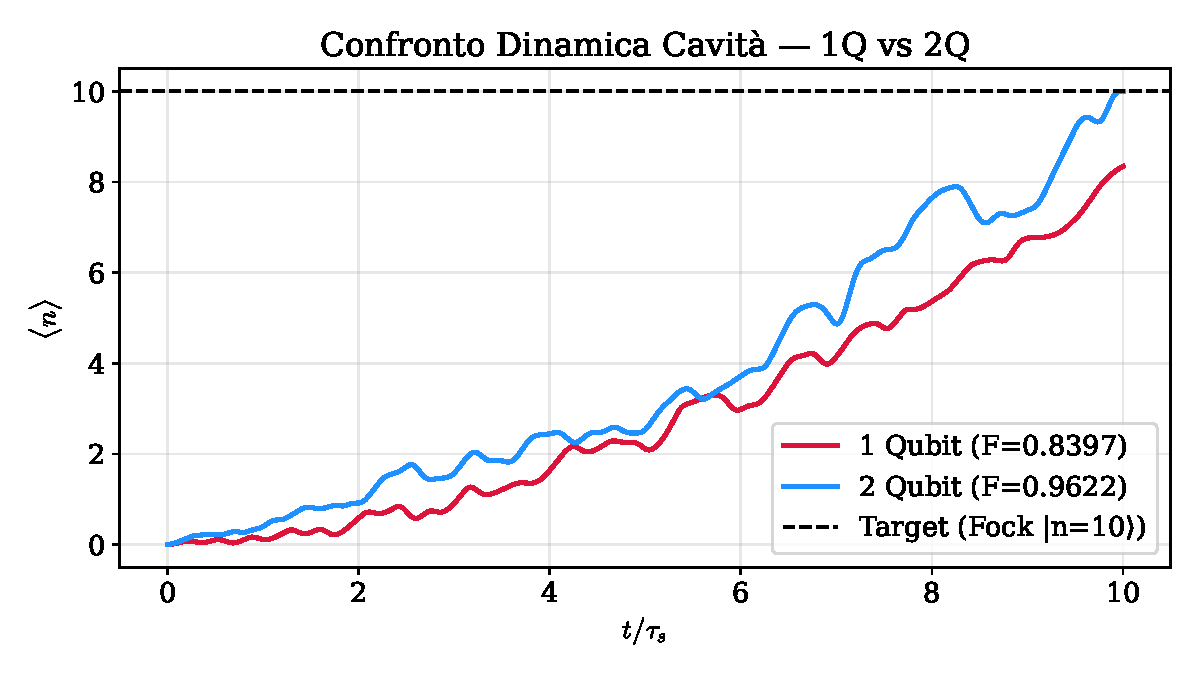
\includegraphics[width=\textwidth]{figure/v1_fock10_t10_comparison_nmean.pdf}
        \caption{Numero medio di fotoni $\langle n \rangle(t)$: 1Q vs 2Q}
    \end{subfigure}
    \hfill
    \begin{subfigure}[b]{0.48\textwidth}
        \centering
        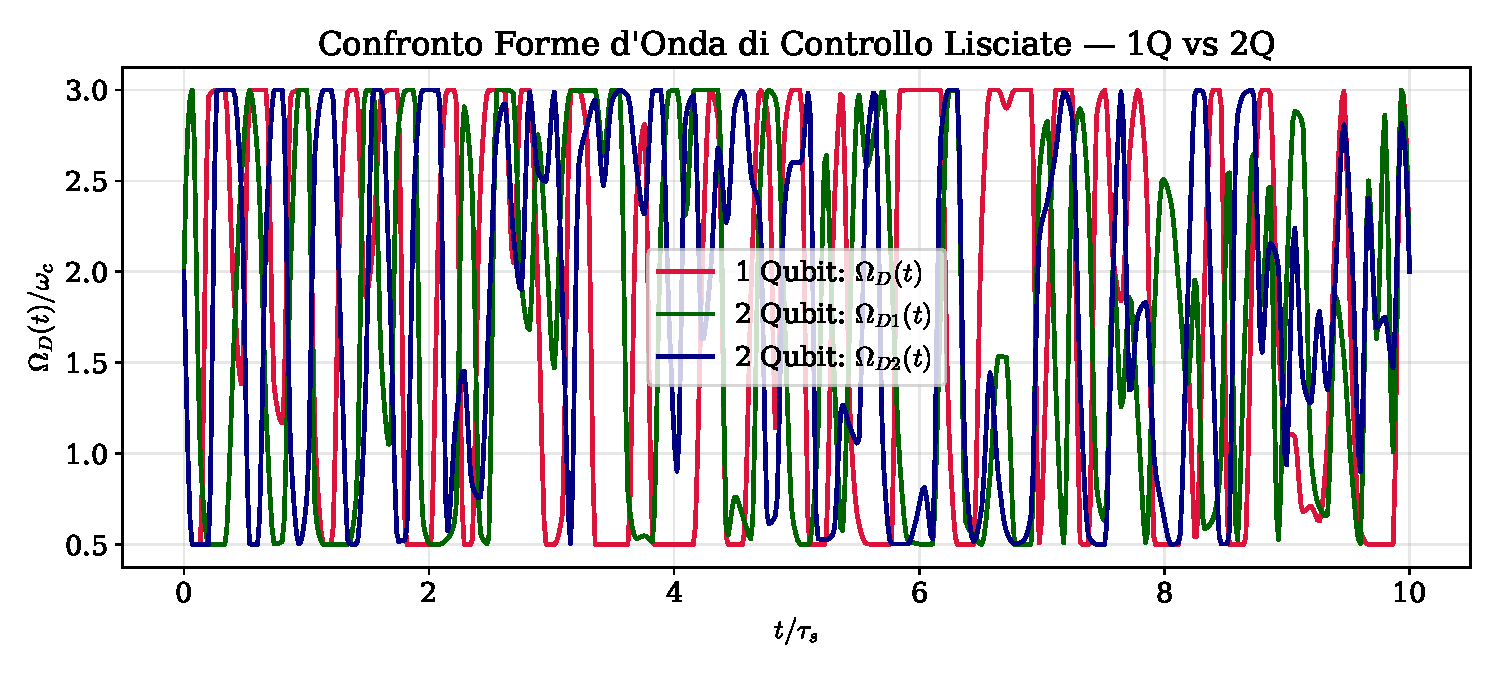
\includegraphics[width=\textwidth]{figure/v1_fock10_t10_comparison_drives.pdf}
        \caption{Controlli ottimali $\Omega_D(t)$ dopo PCHIP: 1Q vs 2Q}
    \end{subfigure}
\end{figure}

\begin{figure}[H]
    \centering
    \begin{subfigure}[b]{0.48\textwidth}
        \centering
        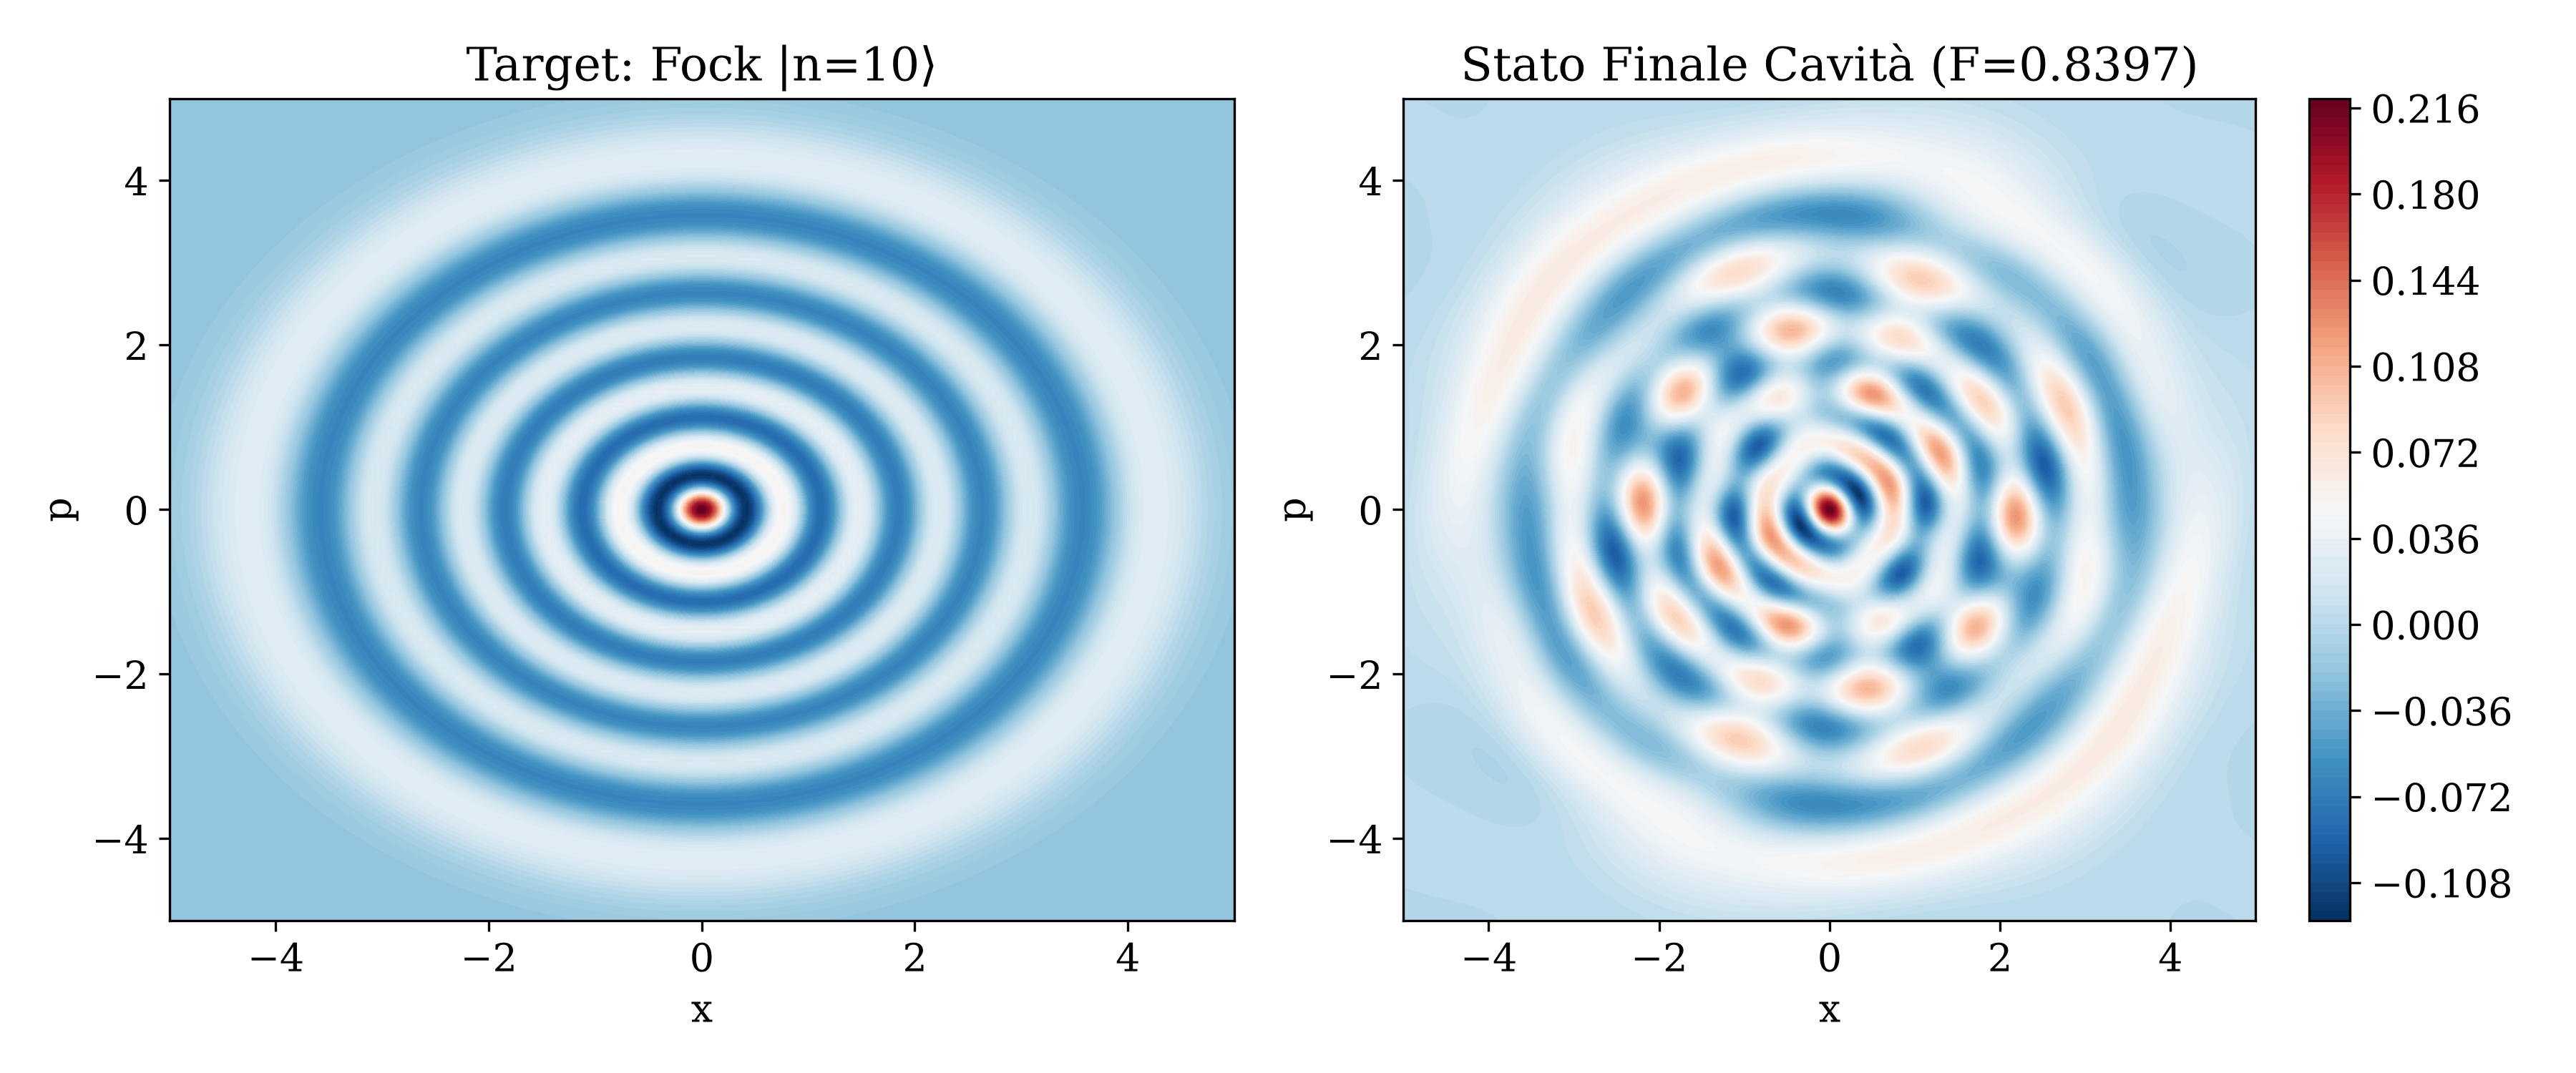
\includegraphics[width=\textwidth]{figure/v1_fock10_t10_1q_wigner.png}
        \caption{1Q ($T=10\,\tau_s$): $F_{\text{smooth}} = 0.8397$ (GRAPE $0.8720$)}
    \end{subfigure}
    \hfill
    \begin{subfigure}[b]{0.48\textwidth}
        \centering
        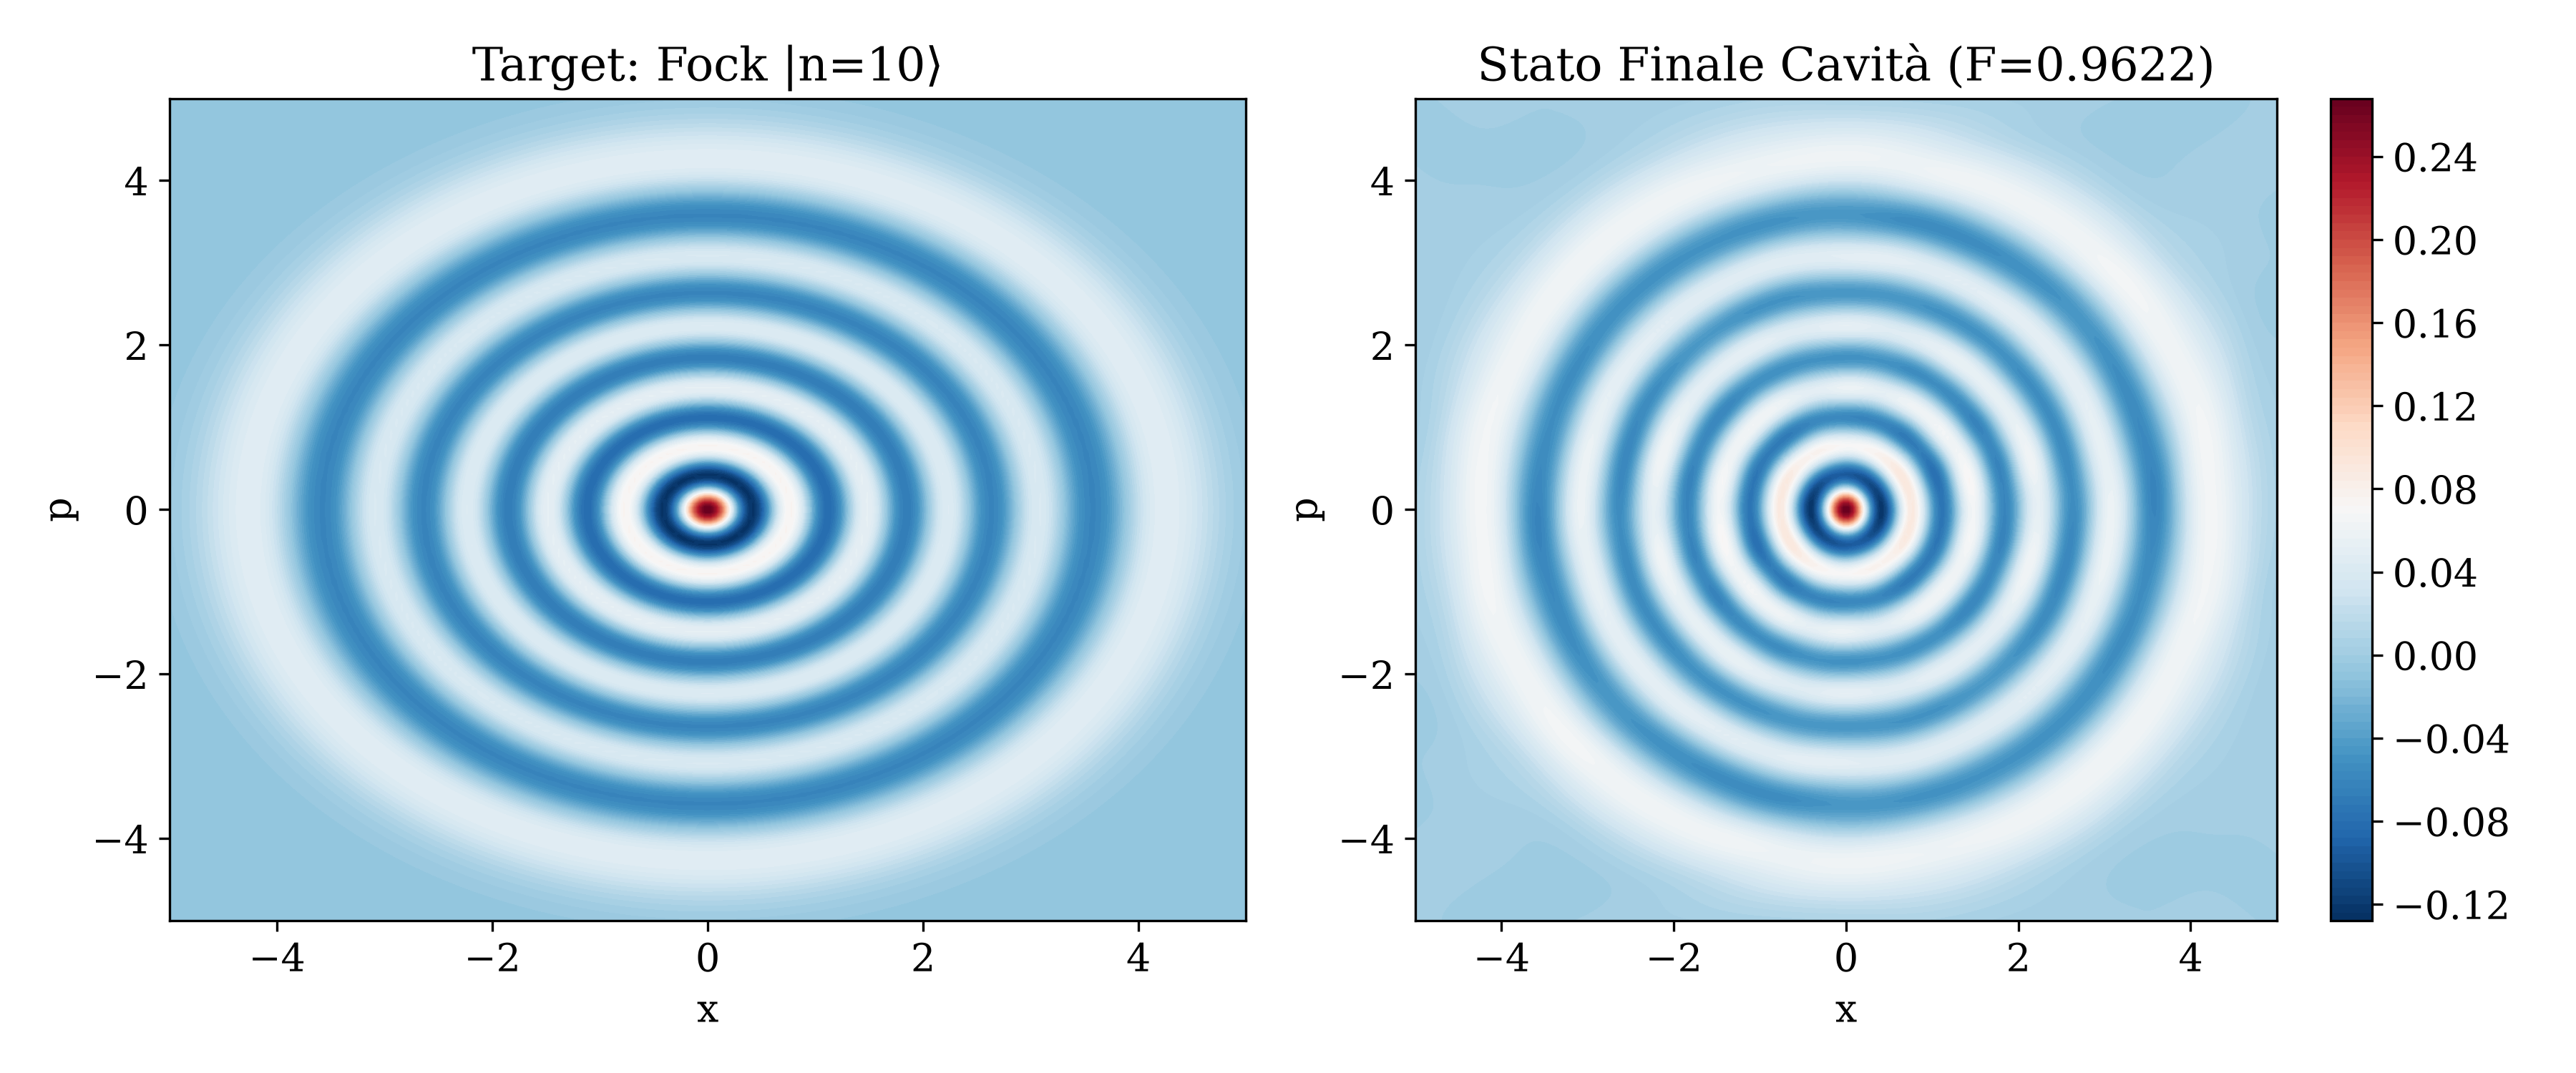
\includegraphics[width=\textwidth]{figure/v1_fock10_t10_2q_wigner.png}
        \caption{2Q ($T=10\,\tau_s$): $F_{\text{smooth}} = 0.9622$ (GRAPE $0.9988$)}
    \end{subfigure}
\end{figure}

\paragraph{2. Confronto 1Q vs 2Q sullo stato Cat a 4 componenti ($\alpha = 2.0$, $T=15\,\tau_s$):}
Nella run \texttt{run\_2026-10-03\_15-06-31} ho confrontato 1Q e 2Q sulla preparazione degli stati Cat con $\alpha = 2.0$ a $T = 15\,\tau_s$ (8 seed CRAB, 150 slot GRAPE).
Qui nella fase GRAPE entrambi i sistemi raggiungevano una fedeltà sopra $0.999$, con slew rate più bassi sui due canali di 2Q ($\text{SR}_{\max} = 5.12$ e $6.24$ contro $6.33$ di 1Q). Tuttavia, appena applicata l'interpolazione PCHIP finale per rendere continuo il controllo a gradini, entrambi i sistemi crollavano di circa il 10\%, scendendo a $0.8945$ (1Q) e $0.8989$ (2Q).

\begin{figure}[H]
    \centering
    \begin{subfigure}[b]{0.48\textwidth}
        \centering
        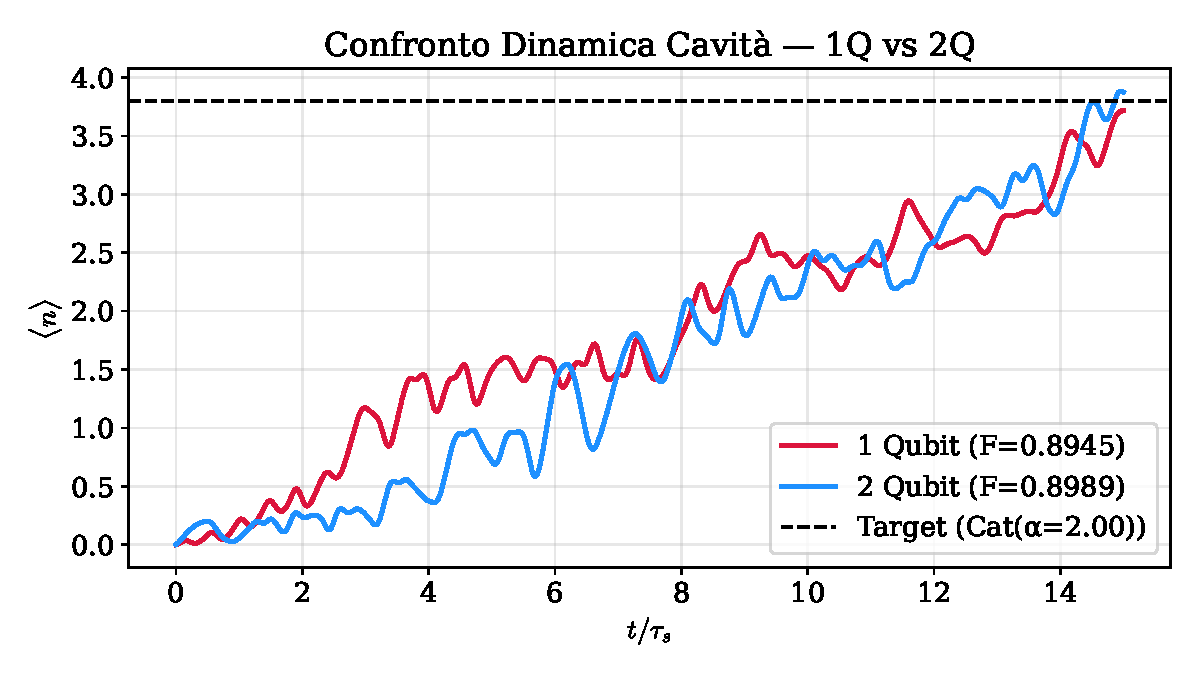
\includegraphics[width=\textwidth]{figure/v1_cat2_t15_comparison_nmean.pdf}
        \caption{Cat $\alpha=2.0$, $T=15\,\tau_s$: evoluzione di $\langle n \rangle(t)$}
    \end{subfigure}
    \hfill
    \begin{subfigure}[b]{0.48\textwidth}
        \centering
        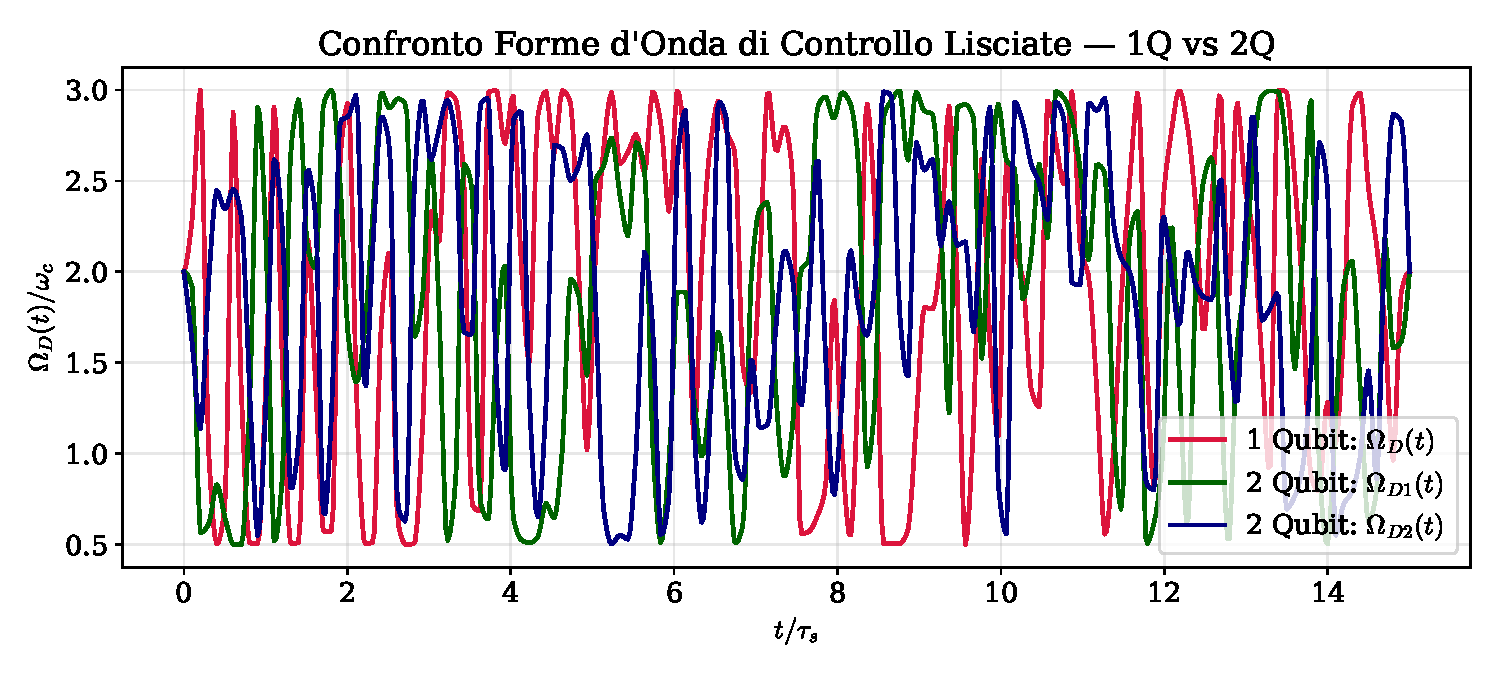
\includegraphics[width=\textwidth]{figure/v1_cat2_t15_comparison_drives.pdf}
        \caption{Cat $\alpha=2.0$, $T=15\,\tau_s$: controlli $\Omega_D(t)$ dopo PCHIP}
    \end{subfigure}
\end{figure}

\begin{figure}[H]
    \centering
    \begin{subfigure}[b]{0.48\textwidth}
        \centering
        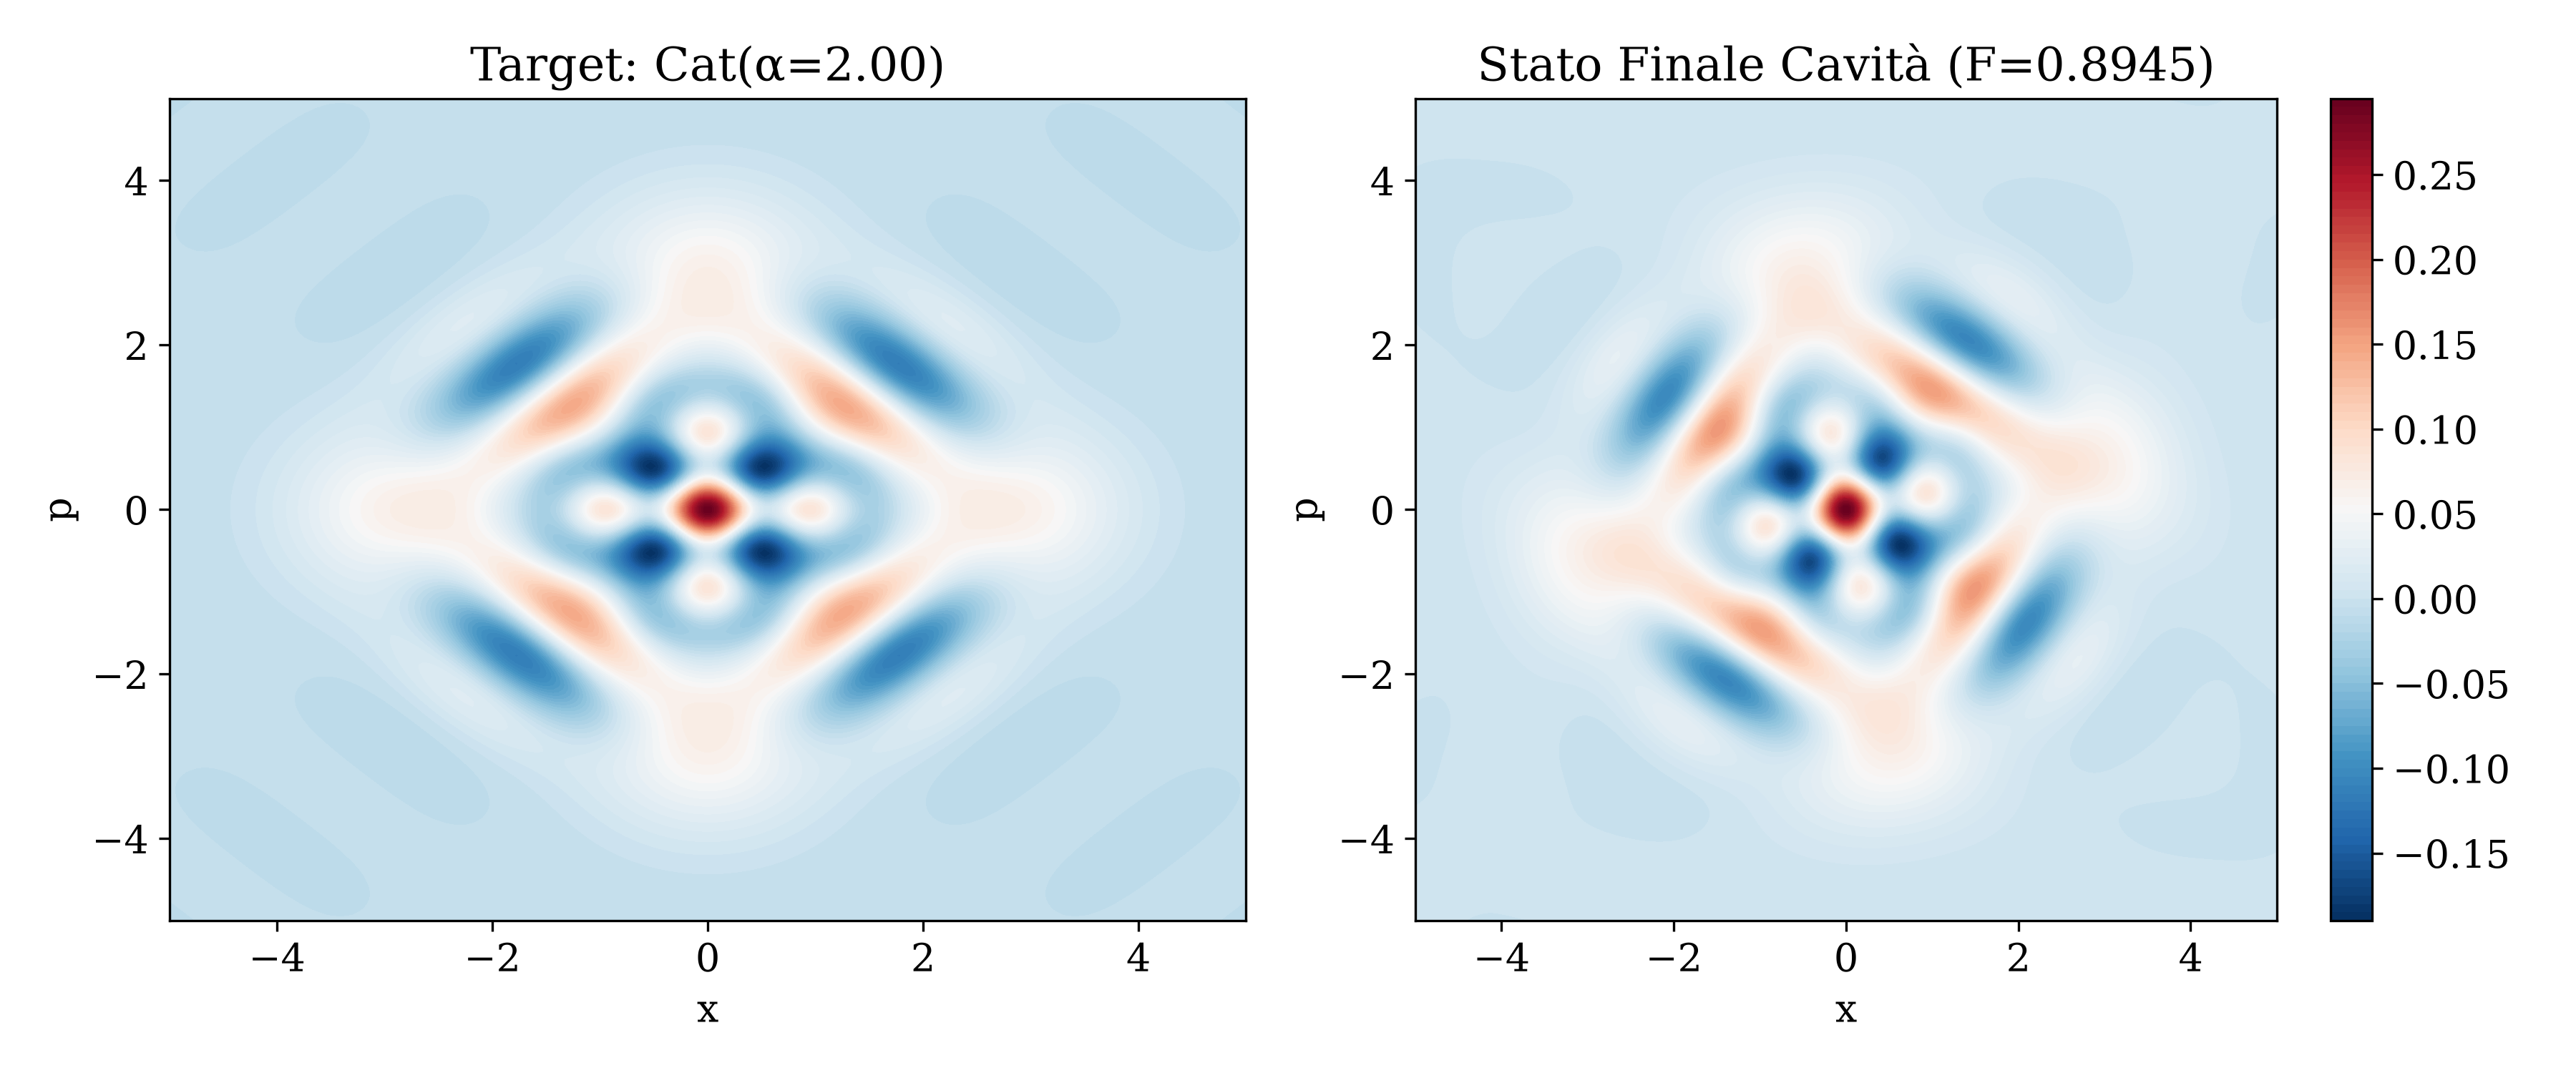
\includegraphics[width=\textwidth]{figure/v1_cat2_t15_1q_wigner.png}
        \caption{1Q ($T=15\,\tau_s$): GRAPE $0.9994 \to$ PCHIP $0.8945$}
    \end{subfigure}
    \hfill
    \begin{subfigure}[b]{0.48\textwidth}
        \centering
        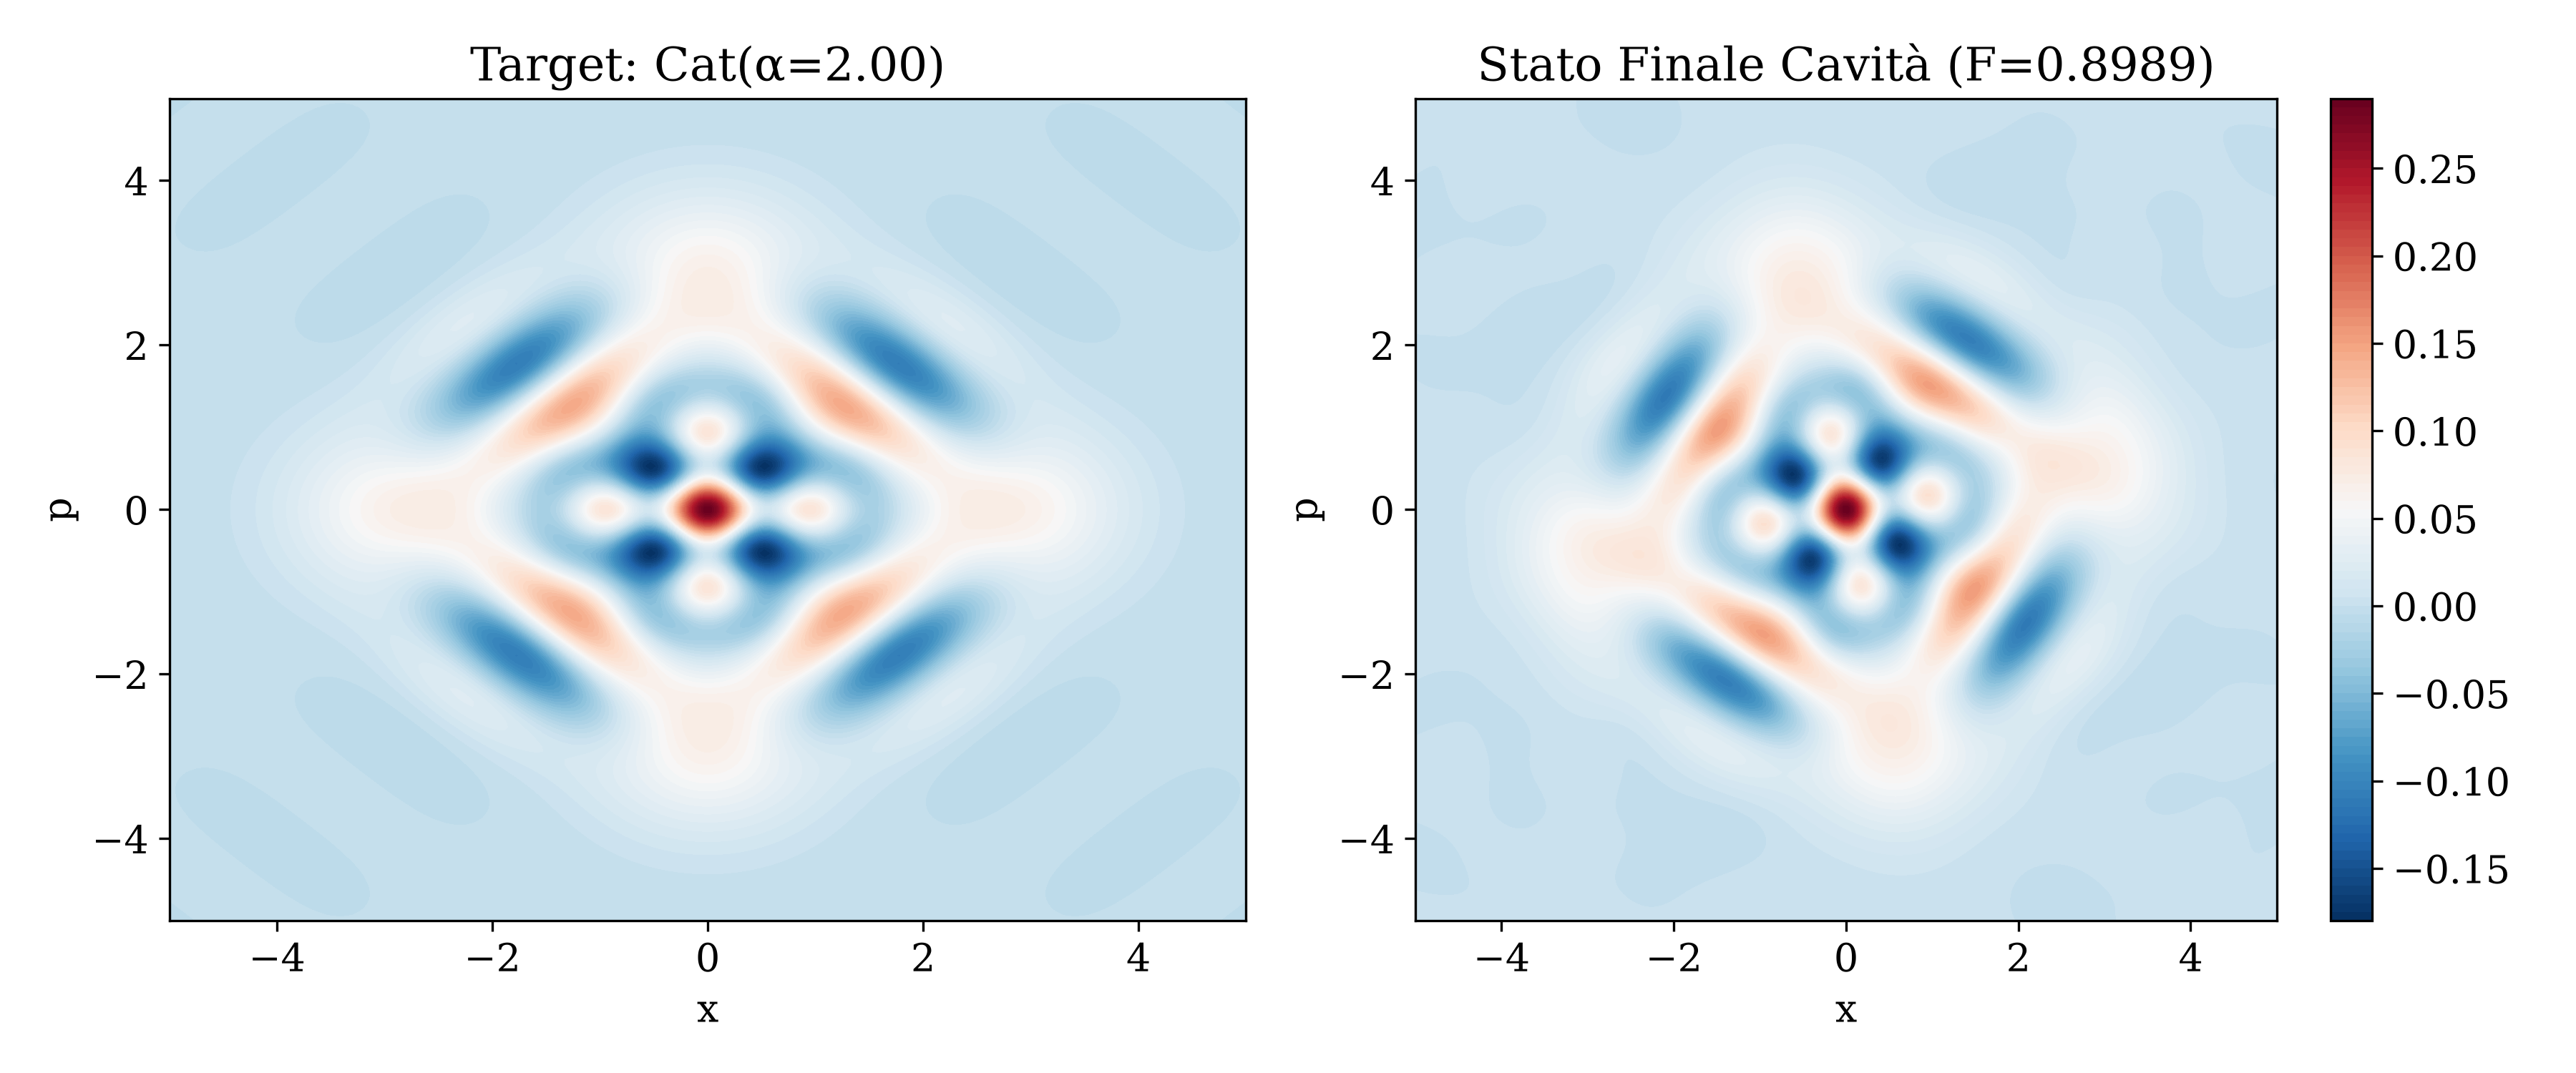
\includegraphics[width=\textwidth]{figure/v1_cat2_t15_2q_wigner.png}
        \caption{2Q ($T=15\,\tau_s$): GRAPE $0.9996 \to$ PCHIP $0.8989$}
    \end{subfigure}
\end{figure}

\subsection{I problemi emersi guardando i risultati della v1}
Analizzando questi risultati ho provato a risolvere alcuni aspetti che ritenevo problematici:
\begin{itemize}
    \item \textbf{Il crollo dopo lo smoothing PCHIP:} ottimizzare un controllo a gradini in GRAPE e lisciarlo solo alla fine cambiava il segnale in modo da far perdere dal 2\% fino al 10\% di fedeltà (come nel caso Cat). In più, anche la verifica del segnale PCHIP veniva fatta ripassandolo al propagatore a gradini su $2 N_t$ punti, e non integrando l'equazione di Schrödinger continua.
    \item \textbf{GRAPE che peggiorava il risultato CRAB (caso 1Q a $T=10\,\tau_s$):} in v1 CRAB integrava con \texttt{sesolve} su 400 punti, mentre GRAPE ricampionava l'impulso su 150 slot costanti a tratti. Inoltre, creando la griglia con \texttt{np.linspace(0, T, Nt)} e applicando $N_t$ passi di durata $dt = T/(N_t - 1)$, l'evoluzione in GRAPE durava in realtà $N_t \cdot T/(N_t-1) > T$. A questo si aggiungeva il fatto che il gradiente era calcolato al primo ordine in $dt$ (usando il commutatore $[H_k, \rho_t]$).
    \item \textbf{Ambiguità nelle metriche:} in CRAB e dopo PCHIP veniva usata \texttt{qutip.fidelity}, che restituisce la radice dell'overlap $F_{\text{root}} = \sqrt{P_{\text{target}}}$, mentre GRAPE massimizzava direttamente la probabilità $P_{\text{target}} = \operatorname{Tr}[O_{\text{target}}\rho]$. Anche il costo $C^2$ integrava la frequenza totale $\Omega_j(t)^2$ (includendo quindi l'offset costante $\omega_q = 2$) invece della sola modulazione.
    \item \textbf{Mancanza di controlli sul troncamento di Fock:} con $n=10$ e $\text{dim}=40$, non era sicuro che la dimensione dello spazio fosse abbastanza grande per non imbattersi in effetti di troncamento.
\end{itemize}

\newpage
\section{Cosa ho cambiato nella v2 e perché}

Per risolvere questi punti ho rivisto la pipeline da zero nella cartella autonoma \texttt{v2/} (lasciando intatti tutti i file e i risultati della v1), implementando diversi test automatici per validare i risultato ottenuti.
\begin{table}[H]
\centering
\small
\renewcommand{\arraystretch}{1.25}
\begin{tabular}{>{\raggedright\arraybackslash}p{2.6cm} >{\raggedright\arraybackslash}p{3.9cm} >{\raggedright\arraybackslash}p{4.3cm} >{\raggedright\arraybackslash}p{3.5cm}}
\toprule
\textbf{Aspetto} & \textbf{Come funzionava in v1} & \textbf{Come funziona in v2} & \textbf{Motivazione} \\
\midrule
\textbf{Forma del controllo e filtro} & Costante a tratti in GRAPE + smoothing PCHIP applicato solo a fine corsa. & Comando lineare a tratti su $M$ nodi (con estremi $\delta(0)=\delta(T)=0$) passato in un filtro causale del 1° ordine ($\omega_{\text{cut}} = 3.0$) calcolato analiticamente. & L'ottimizzatore modifica direttamente il segnale continuo filtrato. Sparisce la perdita da smoothing a posteriori. \\
\addlinespace
\textbf{Griglia temporale e propagazione} & Matrici densità complete; $N_t$ passi di ampiezza $T/(N_t-1)$. & Ket ridotti al settore di parità iniziale (dimensione dimezzata); $N$ intervalli midpoint di passo esatto $dt = T/N$. & L'evoluzione termina esattamente a $T$ ed è molto più veloce in memoria e calcolo. \\
\addlinespace
\textbf{Gradiente GRAPE} & Approssimazione al primo ordine nel passo $dt$ tramite commutatore. & Derivata esatta (Fréchet) dell'esponenziale di matrice nella base degli autovettori di ciascun passo. & \texttt{L-BFGS-B} riceve il gradiente esatto del costo discretizzato e conserva sempre il miglior punto visitato. \\
\addlinespace
\textbf{Validazione numerica} & Assente (solo rivalutazione a gradini su $2 N_t$ punti). & Propagazione continua indipendente (\texttt{sesolve}) confrontata con midpoint a $N$ e $2N$ passi (\texttt{time\_grid}), tolleranze ridotte di $10\times$ e dimensione aumentata di $+20$ livelli. & Un risultato viene accettato solo se il segnale continuo riproduce la fedeltà discreta e non risente del troncamento di Fock. \\
\addlinespace
\textbf{Definizione di fedeltà} & Mista tra $P_{\text{target}}$ e $\sqrt{P_{\text{target}}}$. & Salvataggio separato di $P_{\text{target}}$ e $F_{\text{root}} = \sqrt{P_{\text{target}}}$. Soglia di successo ($0.99$) posta su $P_{\text{target}}$. & Evita ambiguità tra probabilità e radice della probabilità. \\
\addlinespace
\textbf{Statistica sui seed e casi} & 1Q vs 2Q; solo il miglior seed CRAB veniva passato a GRAPE. & 5 casi fisici confrontati; tutti gli 8 seed vengono raffinati con GRAPE. & Valuta la frequenza di successo reale e separa accoppiamento collettivo e numero di canali. \\
\bottomrule
\end{tabular}
\end{table}

\subsection*{Nota sul calcolo esatto del gradiente (derivata di Fréchet)}
Nel propagatore midpoint della v2, su ciascun intervallo temporale $k$ di ampiezza $dt = T/N$ l'Hamiltoniana è costante a tratti, $H_k = H_0 + \sum_j u_{j,k} H_{c,j}$, e il passo di evoluzione è $U_k = e^{-i\,dt\,H_k}$. Per calcolare il gradiente rispetto all'ampiezza di controllo $u_{j,k}$ serve la derivata dell'esponenziale di matrice $\partial U_k / \partial u_{j,k}$.

\noindent
Poiché l'operatore di controllo $H_{c,j}$ (proporzionale a $\sigma_z$) non commuta con l'Hamiltoniana totale $H_k$ (che contiene i termini di scambio fotonico $\sigma_x(a+a^\dagger)$), non vale la regola scalare $\frac{\partial}{\partial u}e^{-i\,dt\,H_k} = -i\,dt\,H_{c,j} U_k$. Nella v1 veniva usata proprio questa approssimazione al primo ordine in $dt$ (tramite il commutatore $[H_{c,j}, \rho_k]$), che però trascura tutti i termini di ordine $\mathcal{O}(dt^2)$ legati alla non-commutatività durante il passo $dt$ e introduce un errore sistematico nella direzione di discesa di \texttt{L-BFGS-B}.

\noindent
Nella v2 ho invece implementato la derivata di Fréchet esatta dell'esponenziale di matrice sfruttando la diagonalizzazione $H_k = V_k \operatorname{diag}(E_a) V_k^\dagger$ già calcolata per propagare lo stato. Nella base degli autovettori istantanei di $H_k$, gli elementi di matrice della derivata esatta hanno la forma chiusa (formula di Daleckii--Krein):
\begin{equation}
    \left(V_k^\dagger \frac{\partial U_k}{\partial u_{j,k}} V_k\right)_{ab} = \left(V_k^\dagger H_{c,j} V_k\right)_{ab} \cdot G_{ab}, \qquad
    G_{ab} = -i\,dt\,e^{-i\,dt\,(E_a + E_b)/2}\,\operatorname{sinc}\!\left(\frac{dt\,(E_a - E_b)}{2\pi}\right),
\end{equation}
dove $\operatorname{sinc}(x) = \sin(\pi x)/(\pi x)$ vale $1$ per $x=0$, rendendo l'espressione numericamente stabile anche in presenza di autovalori degeneri ($E_a = E_b$). In questo modo il gradiente delle ampiezze midpoint (poi riportato ai nodi del comando tramite la matrice analitica del filtro) coincide con la derivata esatta della funzione costo discretizzata fino alla precisione di macchina ($\sim 10^{-15}$). Questa formulazione spettrale per il gradiente esatto in GRAPE è descritta in dettaglio in:
\begin{itemize}
    \item S.~Machnes \emph{et al.}, \emph{``Comparing, Optimizing, and Benchmarking Quantum-Control Algorithms in a Unifying Programming Framework''}, Phys.\ Rev.\ A \textbf{84}, 022305 (2011) — disponibile su arXiv: \href{https://arxiv.org/abs/1011.4874}{\texttt{arXiv:1011.4874}} (Appendice~A / Sez.~II.B sulla derivata esatta dell'esponenziale tramite autodecomposizione);
    \item P.~de~Fouquieres, S.~G.~Schirmer, S.~J.~Glaser, I.~Kuprov, \emph{``Second order gradient ascent pulse engineering''}, J.\ Magn.\ Reson.\ \textbf{212}, 412--417 (2011) — disponibile su arXiv: \href{https://arxiv.org/abs/1102.4096}{\texttt{arXiv:1102.4096}} (mostra perché il gradiente approssimato al primo ordine blocca la convergenza di \texttt{L-BFGS-B} e ricava la derivata esatta del propagatore).
\end{itemize}

\noindent
(Articoli di riferimento, ho utilizzato gemini per capire se e come implementarli nel nostro caso).

\subsection*{Scelta della funzione obiettivo \texttt{root} e configurazione dei 5 casi}
Ho notato che con stati di Fock ad alto numero di fotoni (come $|n=10\rangle$) partendo dal vuoto $|0,g\rangle$, all'inizio della ricerca la probabilità di occupazione del target $P_{\text{target}}$ è prossima a zero ($\sim 10^{-8}$). Usando la funzione costo lineare nella probabilità $J_{\text{prob}} = 1 - P_{\text{target}}$, in quella regione il gradiente è così piccolo da far fermare subito \texttt{L-BFGS-B} per tolleranza sul gradiente. Per evitare questo blocco ho introdotto nella campagna v2 l'obiettivo radice regolarizzato (\texttt{root}):
\begin{equation}
    J_{\text{root}} = \sqrt{1 + \varepsilon} - \sqrt{P_{\text{target}} + \varepsilon} + \text{penalità}, \qquad \varepsilon = 10^{-12},
\end{equation}
il cui gradiente rispetto ai parametri di controllo è moltiplicato per il fattore:
\begin{equation}
    \frac{\partial J_{\text{root}}}{\partial u} = -\frac{1}{2\sqrt{P_{\text{target}} + \varepsilon}}\,\frac{\partial P_{\text{target}}}{\partial u}.
\end{equation}
Quando $P_{\text{target}} \ll 1$, il fattore $1/(2\sqrt{P_{\text{target}} + \varepsilon})$ amplifica automaticamente la derivata senza alterare la direzione del gradiente né la posizione degli ottimi (mentre le metriche salvate nei report restano sempre $P_{\text{target}}$ e $F_{\text{root}} = \sqrt{P_{\text{target}}}$ senza regolarizzazione). Inoltre ho alzato lo spazio di Fock a $\text{dim}=60$ (con verifica di convergenza a $\text{dim}=80$) e il budget a 6000 valutazioni CRAB e 600 iterazioni GRAPE.

\medskip
\noindent
Per rendere equo il confronto tra uno e due qubit, ogni esperimento in v2 mette a confronto 5 configurazioni:
\begin{enumerate}
    \item \texttt{1q}: un qubit con $g = 0.3$;
    \item \texttt{2q\_common}: due qubit con $g_1 = g_2 = 0.3$ pilotati dallo stesso segnale di modulazione (1 canale);
    \item \texttt{2q\_independent}: due qubit con $g_1 = g_2 = 0.3$ pilotati da due segnali indipendenti (2 canali);
    \item \texttt{2q\_normalized\_common}: due qubit con $g_1 = g_2 = 0.3/\sqrt{2} \approx 0.2121$ (così $\sqrt{g_1^2+g_2^2} = 0.3$ come in 1Q) e 1 canale comune;
    \item \texttt{2q\_normalized\_independent}: due qubit con $g_1 = g_2 = 0.3/\sqrt{2}$ e 2 canali indipendenti.
\end{enumerate}

\subsection*{Paragone del costo energetico del controllo vs fluenza (richiesto da Maristella)}
Alla fine di pagina~2 del paper ad un solo qubit, per quantificare il costo energetico dei campi di controllo viene introdotto il funzionale:
\begin{equation}
    C_2(T) := \int_0^T ds\,\|H_D(s)\|_2^2, \qquad \|X\|_2 = \sqrt{\operatorname{Tr}[X^\dagger X]},
\end{equation}
per l'Hamiltoniana di pilotaggio $H_D(t) = \frac{\Omega_D(t)}{2}\sigma_z$. Poiché nello spazio $2\times 2$ del singolo qubit vale $\sigma_z^2 = \mathbb{I}_2$ e $\operatorname{Tr}[\sigma_z^2] = 2$, la norma di Frobenius al quadrato dell'operatore di drive su un singolo qubit è:
\begin{equation}
    \|H_{D,j}(t)\|_2^2 = \operatorname{Tr}_{\mathcal{H}_q}\!\left[\left(\frac{\Omega_{D,j}(t)}{2}\sigma_z\right)^{\!2}\right] = \frac{\Omega_{D,j}(t)^2}{4}\operatorname{Tr}[\mathbb{I}_2] = \frac{1}{2}\Omega_{D,j}(t)^2.
\end{equation}
Di conseguenza, rispetto alla fluenza di modulazione $\mathcal{F}_{\text{mod}} = \sum_j \int_0^T \Omega_{D,j}(t)^2\,dt$ salvata in v2 (e al costo di controllo di Hilbert--Schmidt normalizzato per la dimensione dello spazio di spin, $\frac{1}{d_q}\operatorname{Tr}[H_D^2] = \frac{1}{4}\mathcal{F}_{\text{mod}}$), il funzionale $C_2$ del paper differisce esattamente per un fattore $1/2$ (e sottrae l'offset statico $\omega_q = 2\omega_c$, che invece nella v1 veniva incluso in $\int \Omega_{\text{tot}}(t)^2 dt$ aggiungendo un contributo passivo $\omega_q^2 T \approx 418.9$ a $T=20\,\tau_s$):
\begin{equation}
    C_{2,\text{ch}}^{(j)} = \frac{1}{2}\int_0^T \Omega_{D,j}(t)^2\,dt = \frac{1}{2}\mathcal{F}_{\text{mod}}^{(j)}, \qquad
    C_{2,\text{tot}} = \sum_{j} C_{2,\text{ch}}^{(j)} = \frac{1}{2}\mathcal{F}_{\text{mod,tot}}.
\end{equation}
Con questa convenzione (senza moltiplicare per la dimensione di troncamento artificiale della cavità $\operatorname{Tr}[\mathbb{I}_{\text{cav}}] = \text{dim}$ né per le identità degli altri qubit, così da mantenere la metrica \emph{setup-independent} come dichiarato nel paper), i valori ottenuti per 1Q a $T=20\,\tau_s$ ($C_2/\omega_c^2 \approx 13.6$ per $n=2$, $20.9$ per $n=6$, $26.4$ per $n=10$) coincidono esattamente con la scala $C_2/\omega_c^2 \approx 15\text{--}35$ riportata nella Fig.~3(b) del paper per i protocolli GRAPE. In ogni caso, sia $C_2$ sia la fluenza misurano l'energia matematica integrata dell'impulso di frequenza ($\propto \omega_c^2 T$).

\section{Risultati completi della campagna v2}

La campagna principale comprende 320 pipeline (8 seed $\times$ 5 sistemi $\times$ 8 esperimenti), precedute da una fase di collaudo (\texttt{pilot\_000}--\texttt{pilot\_003} su seed disgiunti $\{100,101\}$, che ha selezionato il profilo \texttt{root\_std0.1}):
\begin{itemize}
    \item \textbf{Blocco filtrato ($\omega_{\text{cut}} = 3.0$):} stati di Fock $n = 2, 6, 10$ a due durate, $T = 10\,\tau_s$ ($1000$ intervalli, $101$ nodi) e $T = 20\,\tau_s$ ($2000$ intervalli, $201$ nodi).
    \item \textbf{Blocco diagnostico senza filtro ($\omega_{\text{cut}} = \text{null}$):} stato di Fock $n = 10$ a $T = 10\,\tau_s$ e $T = 20\,\tau_s$, per isolare quanto del limite a tempi brevi dipenda dal filtro passa-basso e quanto dalla dinamica intrinseca del sistema.
\end{itemize}

\begin{figure}[H]
    \centering
    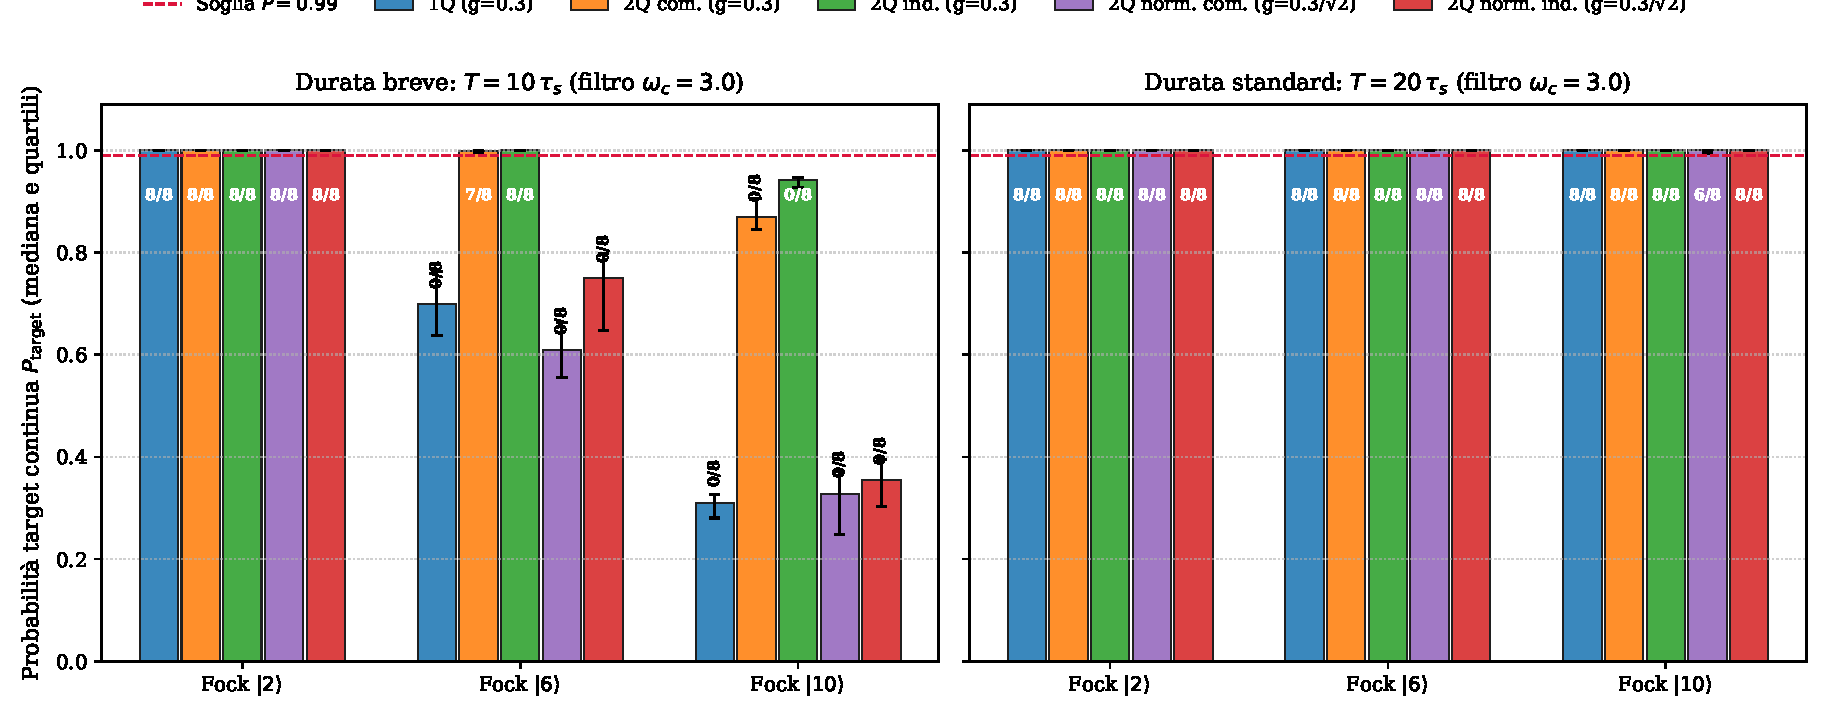
\includegraphics[width=\textwidth]{figure/fig1_panoramica_campagna.pdf}
    \caption{Panoramica dei 6 blocchi principali con filtro causale ($\omega_{\text{cut}}=3.0$): probabilità target continua $P_{\text{target}}$ (mediana e intervallo interquartile su 8 seed) a durata breve $T=10\,\tau_s$ (\texttt{main\_004}, \texttt{main\_006}, \texttt{main\_008}, a sinistra) e a durata standard $T=20\,\tau_s$ (\texttt{main\_005}, \texttt{main\_007}, \texttt{main\_009}, a destra).}
    \label{fig:panoramica_campagna}
\end{figure}

\begin{table}[H]
\centering
\scriptsize
\setlength{\tabcolsep}{3.2pt}
\renewcommand{\arraystretch}{1.13}
\resizebox{\textwidth}{!}{%
\begin{tabular}{llccccccc}
\toprule
\textbf{Esperimento} & \textbf{Sistema} & \textbf{Successi} & \textbf{$P_{\text{target}}$ med.} & \textbf{$P_{\text{target}}$ $[\min, \max]$} & \textbf{Fluenza $\mathcal{F}_{\text{mod}}$} & \textbf{Costo paper $C_2/\omega_c^2$} & \textbf{$\text{SR}_{\max}$ / $\omega_{99\%}$} & \textbf{Validazione numerica} \\
 & & \textbf{validati} & & & \textbf{tot (max ch)} & \textbf{tot (max ch)} & \textbf{(mediana)} & \\
\midrule
\multirow{5}{*}{\shortstack[l]{\textbf{Fock $n=2$, $T=10\,\tau_s$}\\filtro $3.0$ (\texttt{main\_004})}}
 & \texttt{1q} & \textbf{8/8} & 0.999997 & $[0.999996, 0.999998]$ & $22.27$ ($22.27$) & $11.13$ ($11.13$) & $3.64$ / $4.86$ & 8/8 validati (seed~4: $C_2=12.05$) \\
 & \texttt{2q\_common} & \textbf{8/8} & 0.999996 & $[0.999993, 0.999998]$ & $33.00$ ($16.50$) & $16.50$ ($8.25$) & $3.39$ / $4.20$ & 8/8 validati (seed~7: $C_2=14.87$) \\
 & \texttt{2q\_independent} & \textbf{8/8} & 0.999997 & $[0.999996, 0.999998]$ & $30.82$ ($16.64$) & $15.41$ ($8.32$) & $3.42$ / $4.20$ & 8/8 validati (seed~3: $C_2=17.67$) \\
 & \texttt{2q\_norm\_common} & \textbf{8/8} & 0.999990 & $[0.999693, 0.999996]$ & $40.05$ ($20.03$) & $20.03$ ($10.01$) & $3.62$ / $4.62$ & 8/8 validati (seed~2: $C_2=17.27$) \\
 & \texttt{2q\_norm\_independent} & \textbf{8/8} & 0.999994 & $[0.999991, 0.999996]$ & $36.97$ ($20.04$) & $18.49$ ($10.02$) & $3.63$ / $4.86$ & 8/8 validati (seed~5: $C_2=21.88$) \\
\midrule
\multirow{5}{*}{\shortstack[l]{\textbf{Fock $n=2$, $T=20\,\tau_s$}\\filtro $3.0$ (\texttt{main\_005})}}
 & \texttt{1q} & \textbf{8/8} & 0.999998 & $[0.999997, 0.999998]$ & $27.12$ ($27.12$) & $13.56$ ($13.56$) & $3.03$ / $3.54$ & 8/8 validati (seed~3: $C_2=13.13$) \\
 & \texttt{2q\_common} & \textbf{8/8} & 0.999999 & $[0.999997, 1.000000]$ & $36.21$ ($18.10$) & $18.10$ ($9.05$) & $2.27$ / $3.09$ & 8/8 validati (seed~5: $C_2=17.82$) \\
 & \texttt{2q\_independent} & \textbf{8/8} & 0.999999 & $[0.999999, 0.999999]$ & $22.13$ ($12.56$) & $11.06$ ($6.28$) & $2.22$ / $3.24$ & 8/8 validati (seed~5: $C_2=11.97$) \\
 & \texttt{2q\_norm\_common} & \textbf{8/8} & 0.999997 & $[0.999995, 0.999998]$ & $45.09$ ($22.55$) & $22.55$ ($11.27$) & $3.03$ / $3.48$ & 8/8 validati (seed~1: $C_2=22.15$) \\
 & \texttt{2q\_norm\_independent} & \textbf{8/8} & 0.999997 & $[0.999997, 0.999998]$ & $34.44$ ($20.58$) & $17.22$ ($10.29$) & $3.14$ / $3.42$ & 8/8 validati (seed~4: $C_2=15.28$) \\
\midrule
\multirow{5}{*}{\shortstack[l]{\textbf{Fock $n=6$, $T=10\,\tau_s$}\\filtro $3.0$ (\texttt{main\_006})}}
 & \texttt{1q} & \textbf{0/8} & 0.698929 & $[0.596857, 0.776816]$ & $35.30$ ($35.30$) & $17.65$ ($17.65$) & $3.78$ / $4.38$ & 0/8 (fallisce \texttt{time\_grid}) \\
 & \texttt{2q\_common} & \textbf{7/8} & 0.998268 & $[0.986730, 0.999982]$ & $56.26$ ($28.13$) & $28.13$ ($14.07$) & $3.78$ / $5.10$ & 8/8 validati (seed~7: $C_2=26.27$) \\
 & \texttt{2q\_independent} & \textbf{8/8} & 0.999987 & $[0.999963, 0.999994]$ & $47.25$ ($24.58$) & $23.62$ ($12.29$) & $3.74$ / $5.16$ & 8/8 validati (seed~2: $C_2=21.84$) \\
 & \texttt{2q\_norm\_common} & \textbf{0/8} & 0.609237 & $[0.393262, 0.750650]$ & $78.21$ ($39.10$) & $39.10$ ($19.55$) & $3.78$ / $4.74$ & 0/8 (fallisce \texttt{time\_grid}) \\
 & \texttt{2q\_norm\_independent} & \textbf{0/8} & 0.749373 & $[0.577314, 0.837847]$ & $76.63$ ($39.96$) & $38.32$ ($19.98$) & $3.78$ / $4.62$ & 0/8 (fallisce \texttt{time\_grid}) \\
\midrule
\multirow{5}{*}{\shortstack[l]{\textbf{Fock $n=6$, $T=20\,\tau_s$}\\filtro $3.0$ (\texttt{main\_007})}}
 & \texttt{1q} & \textbf{8/8} & 0.999996 & $[0.999996, 0.999997]$ & $41.78$ ($41.78$) & $20.89$ ($20.89$) & $3.62$ / $4.11$ & 8/8 validati (seed~4: $C_2=18.16$) \\
 & \texttt{2q\_common} & \textbf{8/8} & 0.999997 & $[0.999996, 0.999998]$ & $49.98$ ($24.99$) & $24.99$ ($12.50$) & $3.04$ / $3.60$ & 8/8 validati (seed~5: $C_2=21.48$) \\
 & \texttt{2q\_independent} & \textbf{8/8} & 0.999996 & $[0.999993, 0.999998]$ & $47.15$ ($25.23$) & $23.57$ ($12.62$) & $3.08$ / $3.81$ & 8/8 validati (seed~7: $C_2=18.14$) \\
 & \texttt{2q\_norm\_common} & \textbf{8/8} & 0.999989 & $[0.999982, 0.999992]$ & $93.43$ ($46.72$) & $46.72$ ($23.36$) & $3.72$ / $4.32$ & 8/8 validati (seed~3: $C_2=54.03$) \\
 & \texttt{2q\_norm\_independent} & \textbf{8/8} & 0.999993 & $[0.999989, 0.999994]$ & $85.54$ ($48.05$) & $42.77$ ($24.03$) & $3.69$ / $4.44$ & 8/8 validati (seed~1: $C_2=38.06$) \\
\midrule
\multirow{5}{*}{\shortstack[l]{\textbf{Fock $n=10$, $T=10\,\tau_s$}\\filtro $3.0$ (\texttt{main\_008})}}
 & \texttt{1q} & \textbf{0/8} & 0.310186 & $[0.271406, 0.352806]$ & $39.50$ ($39.50$) & $19.75$ ($19.75$) & $3.78$ / $4.80$ & 0/8 (fallisce \texttt{time\_grid}) \\
 & \texttt{2q\_common} & \textbf{0/8} & 0.869445 & $[0.802777, 0.936308]$ & $63.45$ ($31.72$) & $31.72$ ($15.86$) & $3.78$ / $5.28$ & 0/8 (fallisce \texttt{time\_grid}) \\
 & \texttt{2q\_independent} & \textbf{0/8} & 0.940965 & $[0.875524, 0.961781]$ & $68.81$ ($35.30$) & $34.40$ ($17.65$) & $3.78$ / $5.22$ & 0/8 (fallisce \texttt{time\_grid}) \\
 & \texttt{2q\_norm\_common} & \textbf{0/8} & 0.328171 & $[0.179080, 0.442175]$ & $72.90$ ($36.45$) & $36.45$ ($18.22$) & $3.78$ / $4.68$ & 0/8 (fallisce \texttt{time\_grid}) \\
 & \texttt{2q\_norm\_independent} & \textbf{0/8} & 0.355114 & $[0.294268, 0.467935]$ & $79.15$ ($41.36$) & $39.58$ ($20.68$) & $3.78$ / $4.56$ & 0/8 (fallisce \texttt{time\_grid}) \\
\midrule
\multirow{5}{*}{\shortstack[l]{\textbf{Fock $n=10$, $T=20\,\tau_s$}\\filtro $3.0$ (\texttt{main\_009})}}
 & \texttt{1q} & \textbf{8/8} & 0.999992 & $[0.999982, 0.999995]$ & $52.87$ ($52.87$) & $26.43$ ($26.43$) & $3.77$ / $4.77$ & 8/8 validati (seed~3: $C_2=25.93$) \\
 & \texttt{2q\_common} & \textbf{8/8} & 0.999996 & $[0.999994, 0.999997]$ & $70.06$ ($35.03$) & $35.03$ ($17.52$) & $3.63$ / $4.11$ & 8/8 validati (seed~0: $C_2=36.59$) \\
 & \texttt{2q\_independent} & \textbf{8/8} & 0.999994 & $[0.999990, 0.999995]$ & $53.52$ ($29.52$) & $26.76$ ($14.76$) & $3.49$ / $4.26$ & 8/8 validati (seed~4: $C_2=26.68$) \\
 & \texttt{2q\_norm\_common} & \textbf{6/8} & 0.999956 & $[0.972811, 0.999985]$ & $111.49$ ($55.74$) & $55.74$ ($27.87$) & $3.77$ / $4.92$ & 6/8 validati (seed~4: $C_2=55.73$) \\
 & \texttt{2q\_norm\_independent} & \textbf{8/8} & 0.999986 & $[0.999984, 0.999993]$ & $102.53$ ($54.35$) & $51.26$ ($27.18$) & $3.75$ / $4.74$ & 8/8 validati (seed~3: $C_2=58.08$) \\
\midrule
\multirow{5}{*}{\shortstack[l]{\textbf{Fock $n=10$, $T=10\,\tau_s$}\\senza filtro (\texttt{main\_010})}}
 & \texttt{1q} & \textbf{0/8} & 0.635531 & $[0.573466, 0.703158]$ & $54.74$ ($54.74$) & $27.37$ ($27.37$) & $4.77$ / $7.80$ & 0/8 (fallisce \texttt{time\_grid}) \\
 & \texttt{2q\_common} & \textbf{2/8} & 0.981896 & $[0.967130, 0.999879]$ & $80.38$ ($40.19$) & $40.19$ ($20.10$) & $4.77$ / $7.98$ & 2/8 validati (seed~7: $C_2=37.25$) \\
 & \texttt{2q\_independent} & \textbf{8/8} & 0.999937 & $[0.999414, 0.999970]$ & $78.46$ ($41.31$) & $39.23$ ($20.65$) & $4.77$ / $7.98$ & 8/8 validati (seed~5: $C_2=36.80$) \\
 & \texttt{2q\_norm\_common} & \textbf{0/8} & 0.561297 & $[0.506857, 0.676184]$ & $98.35$ ($49.17$) & $49.17$ ($24.59$) & $4.77$ / $7.80$ & 0/8 (fallisce \texttt{time\_grid}) \\
 & \texttt{2q\_norm\_independent} & \textbf{0/8} & 0.730965 & $[0.598527, 0.829199]$ & $106.75$ ($55.62$) & $53.38$ ($27.81$) & $4.77$ / $7.74$ & 0/8 (fallisce \texttt{time\_grid}) \\
\midrule
\multirow{5}{*}{\shortstack[l]{\textbf{Fock $n=10$, $T=20\,\tau_s$}\\senza filtro (\texttt{main\_011})}}
 & \texttt{1q} & \textbf{8/8} & 0.999974 & $[0.999967, 0.999979]$ & $55.58$ ($55.58$) & $27.79$ ($27.79$) & $4.70$ / $7.44$ & 8/8 validati (seed~5: $C_2=28.24$) \\
 & \texttt{2q\_common} & \textbf{8/8} & 0.999983 & $[0.999979, 0.999990]$ & $70.82$ ($35.41$) & $35.41$ ($17.71$) & $3.70$ / $5.10$ & 8/8 validati (seed~0: $C_2=37.81$) \\
 & \texttt{2q\_independent} & \textbf{8/8} & 0.999979 & $[0.999974, 0.999987]$ & $49.53$ ($28.53$) & $24.77$ ($14.26$) & $3.97$ / $7.23$ & 8/8 validati (seed~4: $C_2=27.86$) \\
 & \texttt{2q\_norm\_common} & \textbf{8/8} & 0.999978 & $[0.999951, 0.999985]$ & $118.78$ ($59.39$) & $59.39$ ($29.70$) & $4.76$ / $7.23$ & 8/8 validati (seed~2: $C_2=53.93$) \\
 & \texttt{2q\_norm\_independent} & \textbf{8/8} & 0.999972 & $[0.999946, 0.999977]$ & $114.15$ ($61.40$) & $57.08$ ($30.70$) & $4.76$ / $7.38$ & 8/8 validati (seed~5: $C_2=50.67$) \\
\bottomrule
\end{tabular}%
}
\caption{Risultati completi della campagna v2 su tutti gli 8 blocchi principali (\texttt{main\_004}--\texttt{main\_011}). I valori di fluenza di modulazione $\mathcal{F}_{\text{mod}}$, costo del paper $C_2/\omega_c^2 = \mathcal{F}_{\text{mod}}/2$, slew rate massimo $\text{SR}_{\max}$ e banda al 99\% $\omega_{99\%}$ sono le mediane sugli 8 seed (con il valore del seed selezionato indicato nell'ultima colonna).}
\label{tab:risultati_campagna}
\end{table}

\subsection*{Analisi dei dati sul confronto 1Q vs 2Q}

\begin{enumerate}
    \item \textbf{A tempi lunghi ($T = 20\,\tau_s$) tutti i sistemi preparano lo stato, anche 1Q e i casi normalizzati:}
    Sia per $n=2$, sia per $n=6$, sia per $n=10$, a $T=20\,\tau_s$ con filtro attivo il singolo qubit (\texttt{1q}) e i due qubit con accoppiamento normalizzato (\texttt{2q\_normalized\_independent}) centrano l'obiettivo su 8/8 seed, con probabilità certificate superiori a $0.99998$. Soltanto \texttt{2q\_normalized\_common} su $n=10$ fallisce su 2 seed su 8 (fermandosi comunque a $P \approx 0.973 - 0.975$, mentre raggiunge 8/8 senza filtro in \texttt{main\_011}). Quindi, quando il tempo di interazione è $20\,\tau_s$, un singolo qubit è perfettamente in grado di generare anche Fock $|n=10\rangle$ con il filtro attivo.

    \item \textbf{A tempi brevi ($T = 10\,\tau_s$) emerge un vantaggio netto dei 2 qubit, ma legato soprattutto all'accoppiamento collettivo $\sqrt{2}g$:}
    Guardando \texttt{main\_006} (Fock $n=6$ a $T=10\,\tau_s$, Figura~\ref{fig:dinamica_fock6_t10}), i due sistemi con accoppiamento pieno per singolo qubit ($g_1=g_2=0.3$) raggiungono la soglia in modo certificato (\texttt{2q\_independent} con 8/8 seed e mediana $0.999987$; \texttt{2q\_common} con 7/8 seed e mediana $0.998268$). Al contrario, \texttt{1q} si ferma a una mediana di $0.6989$ (0/8), e i due sistemi a due qubit con accoppiamento riscalato $g_j = 0.3/\sqrt{2}$ (\texttt{2q\_normalized\_common} a $0.6092$ e \texttt{2q\_normalized\_independent} a $0.7494$) restano anch'essi a 0/8 su valori molto vicini a \texttt{1q}.
    Lo stesso schema si ripete su Fock $n=10$ a $T=10\,\tau_s$ (\texttt{main\_008} e \texttt{main\_010}): i casi \texttt{2q\_normalized} hanno sempre prestazioni paragonabili a \texttt{1q} e molto lontane da quelle di \texttt{2q\_common} e \texttt{2q\_independent}. Questo mostra chiaramente che la possibilità di dimezzare il tempo di preparazione da $20\,\tau_s$ a $10\,\tau_s$ per stati ad alto numero di fotoni dipende prima di tutto dall'aumento dell'accoppiamento efficace ($\sqrt{g_1^2+g_2^2} = \sqrt{2}g$).

    \begin{figure}[H]
        \centering
        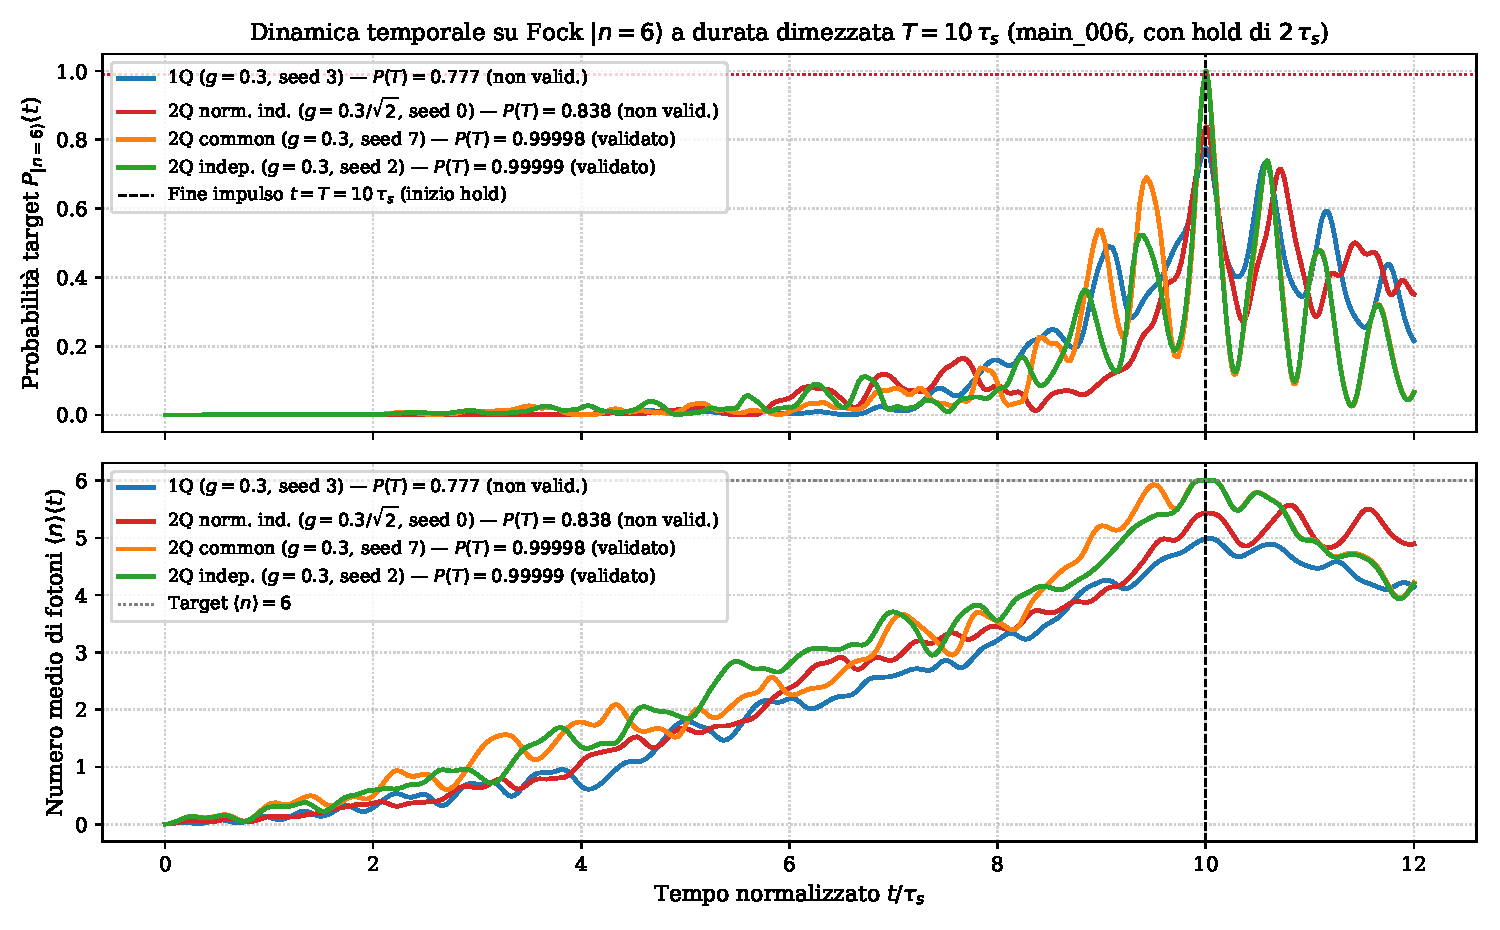
\includegraphics[width=0.95\textwidth]{figure/fig4_dinamica_fock6_t10.pdf}
        \caption{Dinamica temporale della probabilità target $P_{|n=6\rangle}(t)$ (in alto) e del numero medio di fotoni $\langle n \rangle(t)$ (in basso) per Fock $|n=6\rangle$ a durata dimezzata $T = 10\,\tau_s$ (\texttt{main\_006}). è visibile la fase di \texttt{hold\_time} a comando spento, in cui lo stato scambia energia con i qubit a causa dell'accoppiamento $g$ sempre attivo.}
        \label{fig:dinamica_fock6_t10}
    \end{figure}

    \item \textbf{Il ruolo del secondo canale indipendente (\texttt{2q\_independent} vs \texttt{2q\_common}):}
    A parità di accoppiamento fisico ($g_1=g_2=0.3$), avere due controlli indipendenti invece di un controllo comune dà un vantaggio visibile quando il problema diventa più stretto:
    \begin{itemize}
        \item su Fock $n=6$ a $T=10\,\tau_s$ (\texttt{main\_006}), \texttt{2q\_independent} porta a termine 8/8 seed con mediana $0.999987$ contro i 7/8 di \texttt{2q\_common} (mediana $0.998268$);
        \item su Fock $n=10$ a $T=10\,\tau_s$ senza filtro (\texttt{main\_010}, Figura~\ref{fig:filtro_vs_nofiltro}), \texttt{2q\_independent} valida 8/8 seed sopra soglia (mediana $0.999937$), mentre \texttt{2q\_common} si ferma a 2/8 seed validati (mediana $0.981896$).
    \end{itemize}
    Anche a parità di accoppiamento normalizzato ($g_j = 0.3/\sqrt{2}$), \texttt{2q\_normalized\_independent} ottiene sistematicamente mediane più alte di \texttt{2q\_normalized\_common} nei regimi a $10\,\tau_s$ ($0.749$ vs $0.609$ su $n=6$; $0.731$ vs $0.561$ su $n=10$ senza filtro) e 8/8 contro 6/8 su $n=10$ a $20\,\tau_s$. Tuttavia, da solo (senza l'aumento di $g_{\text{eff}}$), il secondo canale non basta a far raggiungere la soglia $0.99$ a $T=10\,\tau_s$ per $n=6$ o $n=10$.

    \item \textbf{L'effetto del filtro passa-basso a $T = 10\,\tau_s$ e $T = 20\,\tau_s$ (\texttt{main\_008}--\texttt{main\_011}):}
    Confrontando \texttt{main\_008} (con filtro $\omega_{\text{cut}}=3.0$) e \texttt{main\_010} (senza filtro) in Figura~\ref{fig:spettro_filtro}, si vede perché a $T=10\,\tau_s$ con filtro nemmeno \texttt{2q\_independent} superava $0.99$ (fermandosi a mediana $0.9410$, max $0.9618$): il filtro con polo a $3\omega_c$ attenua le variazioni rapide sui 101 nodi di comando. Togliendo il filtro (\texttt{main\_010}), \texttt{2q\_independent} sale subito a 8/8 successi validati ($P_{\text{mediana}} = 0.999937$), usando una banda $\omega_{99\%} \approx 7.6 - 8.4\,\omega_c$. Al contrario, a $T=20\,\tau_s$ (\texttt{main\_009} vs \texttt{main\_011}, Figura~\ref{fig:spettro_filtro}b), il filtro $\omega_{\text{cut}}=3.0$ è del tutto vantaggioso: riduce la banda $\omega_{99\%}$ da $\sim 7.2\text{--}8.1\,\omega_c$ a $\sim 4.1\text{--}4.8\,\omega_c$ e lo slew rate da $\sim 4.7$ a $\sim 3.5\text{--}3.8$, mantenendo $P > 0.99999$.

    \begin{figure}[H]
        \centering
        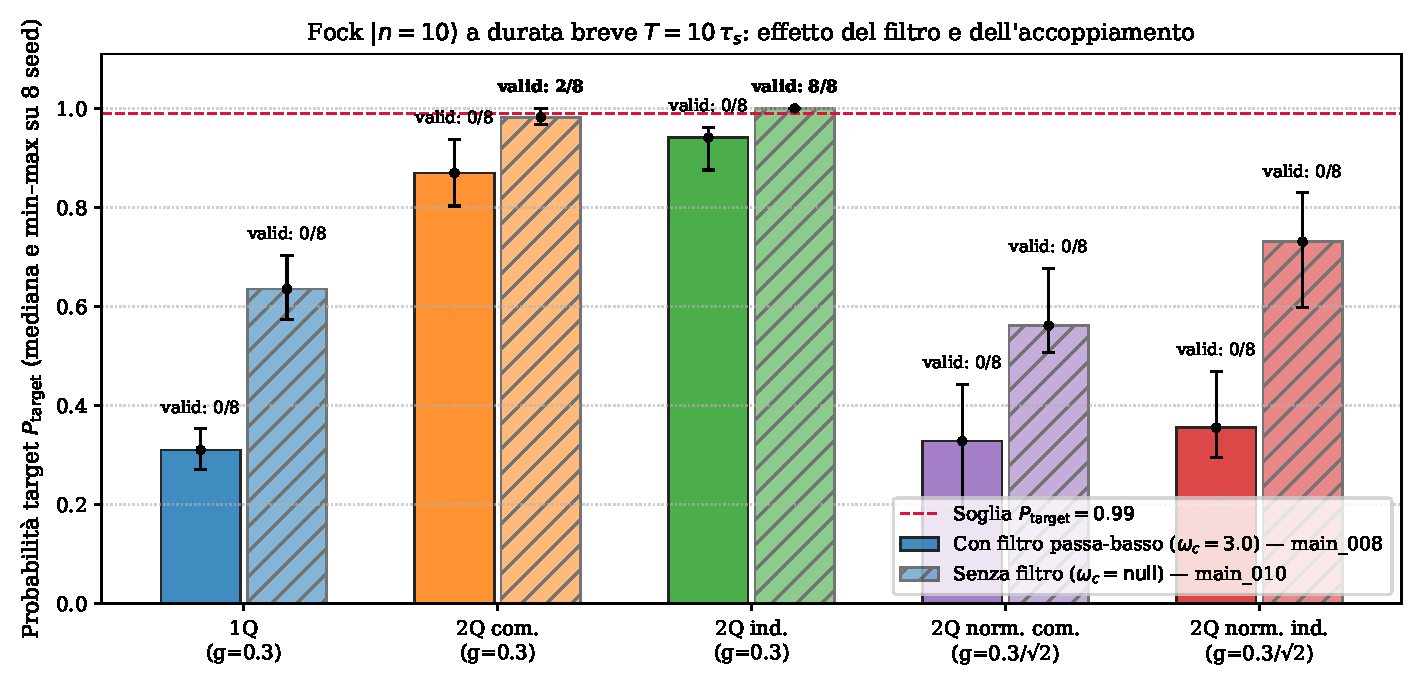
\includegraphics[width=0.90\textwidth]{figure/fig2_fock10_t10_filtro_vs_nofiltro.pdf}
        \caption{Confronto su Fock $|n=10\rangle$ a $T = 10\,\tau_s$ tra il blocco con filtro causale $\omega_{\text{cut}}=3.0$ (\texttt{main\_008}, barre piene) e il blocco senza filtro (\texttt{main\_010}, barre tratteggiate). Togliendo il filtro, \texttt{2q\_independent} passa da 0/8 a 8/8 seed validati sopra soglia ($P_{\text{mediana}} = 0.999937$), mentre \texttt{1q} e i casi \texttt{2q\_normalized} restano sotto $0.83$ anche senza filtro.}
        \label{fig:filtro_vs_nofiltro}
    \end{figure}

    \begin{figure}[H]
        \centering
        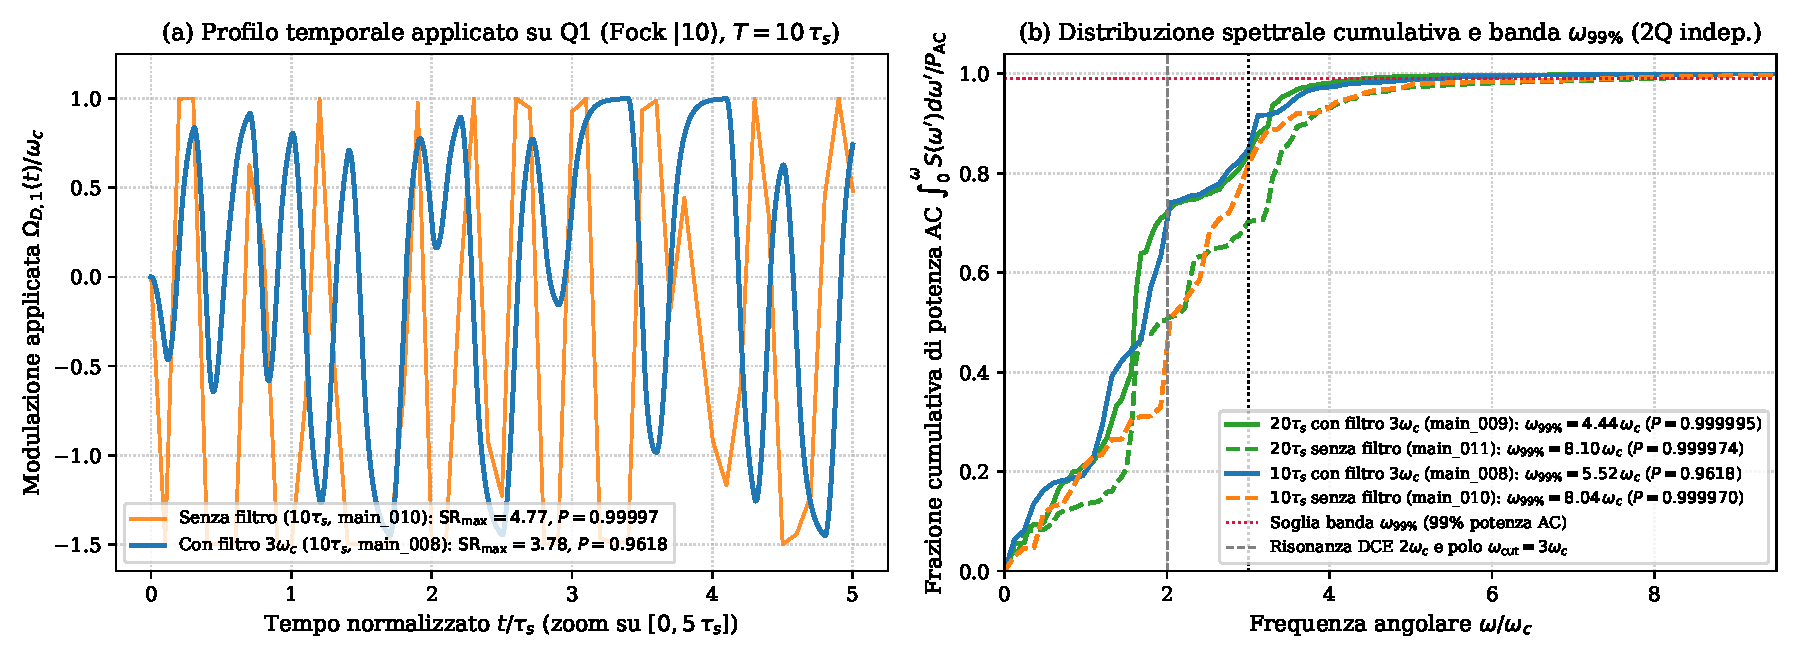
\includegraphics[width=0.96\textwidth]{figure/fig7_spettro_filtro_main009_vs_011.pdf}
        \caption{Effetto del filtro causale ($\omega_{\text{cut}}=3.0\,\omega_c$) su Fock $|n=10\rangle$ per \texttt{2q\_independent}: (a) profilo temporale della modulazione applicata $\Omega_{D,1}(t)$ nei primi $5\,\tau_s$ con e senza filtro; (b) frazione cumulativa della potenza spettrale AC in funzione della frequenza $\omega/\omega_c$, che illustra la riduzione della banda al 99\% ($\omega_{99\%}$) da $\sim 8\,\omega_c$ a $\sim 4.4\text{--}5.5\,\omega_c$.}
        \label{fig:spettro_filtro}
    \end{figure}

    \item \textbf{Costo energetico $C_2$ totale vs per singolo canale (Figura~\ref{fig:scaling_costo_C2}):}
    Confrontando lo scaling del costo energetico $C_2/\omega_c^2$ a $T=20\,\tau_s$ (\texttt{main\_005}, \texttt{main\_007}, \texttt{main\_009} in Figura~\ref{fig:scaling_costo_C2}), si osserva che \texttt{2q\_independent} ($g=0.3$) richiede un costo energetico totale $C_{2,\text{tot}}$ uguale o persino inferiore a quello del singolo qubit \texttt{1q} ($11.1$ contro $13.6$ per $n=2$; $23.6$ contro $20.9$ per $n=6$; $26.8$ contro $26.4$ per $n=10$), ma ripartendolo su due canali riduce del \textbf{$40\%\text{--}54\%$} il carico massimo sulla singola linea di controllo ($C_{2,\text{max ch}} = 6.3$ vs $13.6$ su $n=2$; $12.6$ vs $20.9$ su $n=6$; $14.8$ vs $26.4$ su $n=10$). Nei casi normalizzati ($g=0.3/\sqrt{2}$), invece, per compensare il minore accoppiamento individuale ogni canale deve modulare quanto \texttt{1q} ($C_{2,\text{max ch}} \approx 23\text{--}28$), raddoppiando il costo totale ($C_{2,\text{tot}} \approx 43\text{--}56$).

    \begin{figure}[H]
        \centering
        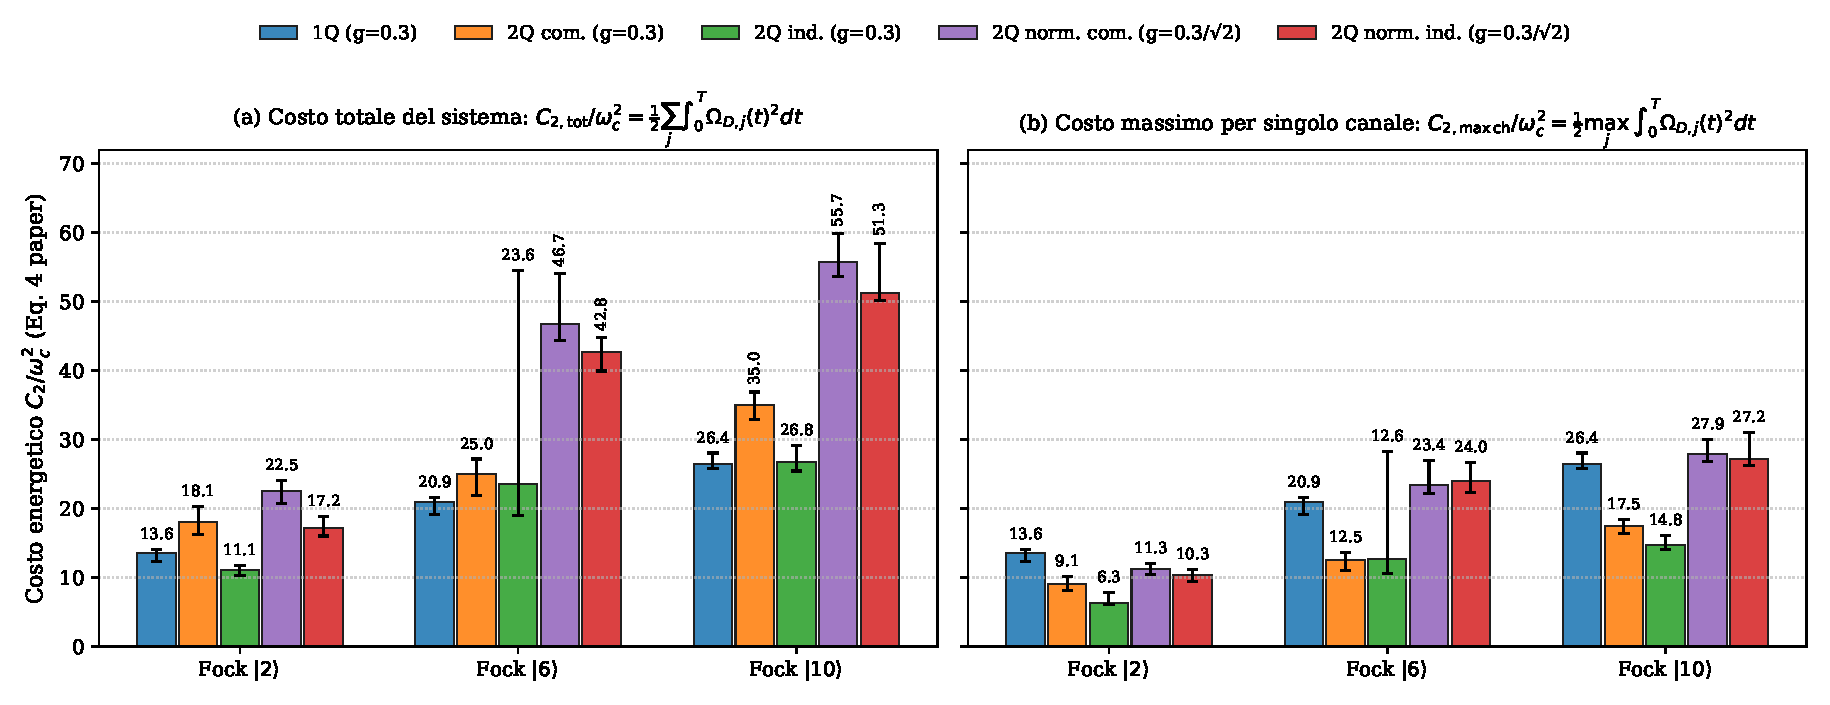
\includegraphics[width=0.98\textwidth]{figure/fig5_scaling_costo_C2.pdf}
        \caption{Scaling del costo energetico di controllo $C_2/\omega_c^2$ (Eq.~4 del paper, mediana e quartili su 8 seed) a $T = 20\,\tau_s$ con filtro $\omega_{\text{cut}}=3.0$ (\texttt{main\_005}, \texttt{main\_007}, \texttt{main\_009}): (a) costo totale del sistema $C_{2,\text{tot}}$ sommato sui canali; (b) costo massimo per singolo canale $C_{2,\text{max ch}}$. Il caso \texttt{2q\_independent} mantiene lo stesso costo totale di \texttt{1q} ma dimezza quasi il carico per singolo canale.}
        \label{fig:scaling_costo_C2}
    \end{figure}

    \item \textbf{Singoletto ``dark'' $|D\rangle$:}
Attivazione dello stato ``dark'' di singoletto $|D\rangle = (|g,e\rangle - |e,g\rangle)/\sqrt{2}$: in \texttt{2q\_common} la popolazione di singoletto è identicamente nulla ($\sim 10^{-21}$) per simmetria di scambio. In \texttt{2q\_independent}, invece, la modulazione differenziale $\Omega_1(t) \neq \Omega_2(t)$ trasferisce fino al $40\text{--}56\%$ della popolazione nello stato antisimmetrico $|D\rangle$ a metà evoluzione, per poi svuotarlo completamente a $t=T$ ($P_{|D\rangle}(T) \sim 10^{-6}$).

    \begin{figure}[H]
        \centering
        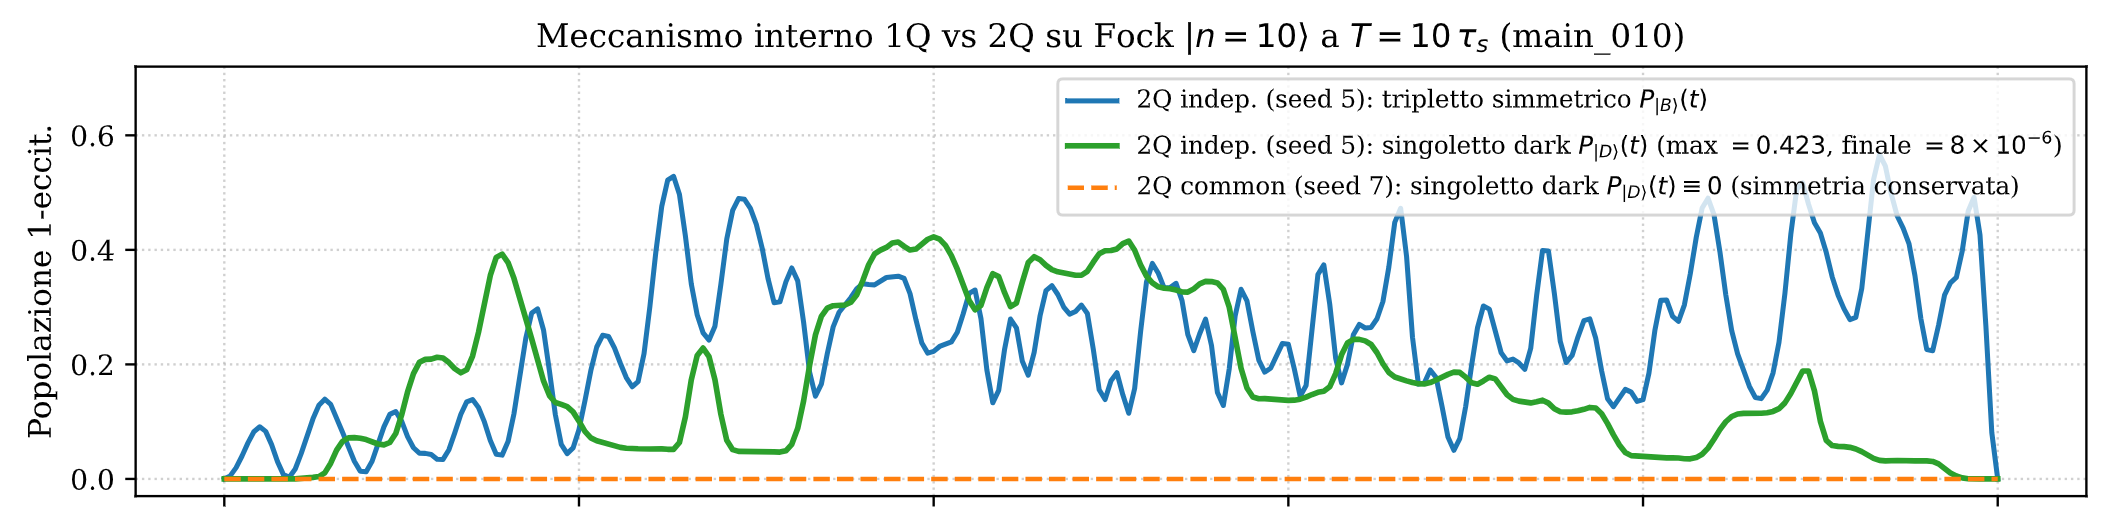
\includegraphics[width=0.95\textwidth]{figure/image.png}
        \caption{Meccanismo fisico interno durante la preparazione di Fock $|n=10\rangle$ a $T=10\,\tau_s$ (\texttt{main\_010}): popolazione del tripletto luminoso $|B\rangle$ e del singoletto dark $|D\rangle$, attivo solo in \texttt{2q\_independent}.}
        \label{fig:meccanismo_dicke}
    \end{figure}
\end{enumerate}

\section{Confronto tra risultati v1 e v2 (e ruolo di CRAB)}

Nella Tabella~\ref{tab:confronto_v1_v2} (e Figura~\ref{fig:confronto_v1_v2}) sono affiancati i casi di Fock simulati sia in v1 sia in v2. In v1 il valore finale riguardava il solo miglior seed dopo smoothing PCHIP a posteriori ($\text{dim}=40$, senza filtro in ottimizzazione); in v2 è la probabilità continua da \texttt{sesolve} su 8 seed tutti raffinati e validati ($\text{dim}=60$ vs $80$).

\begin{figure}[H]
    \centering
    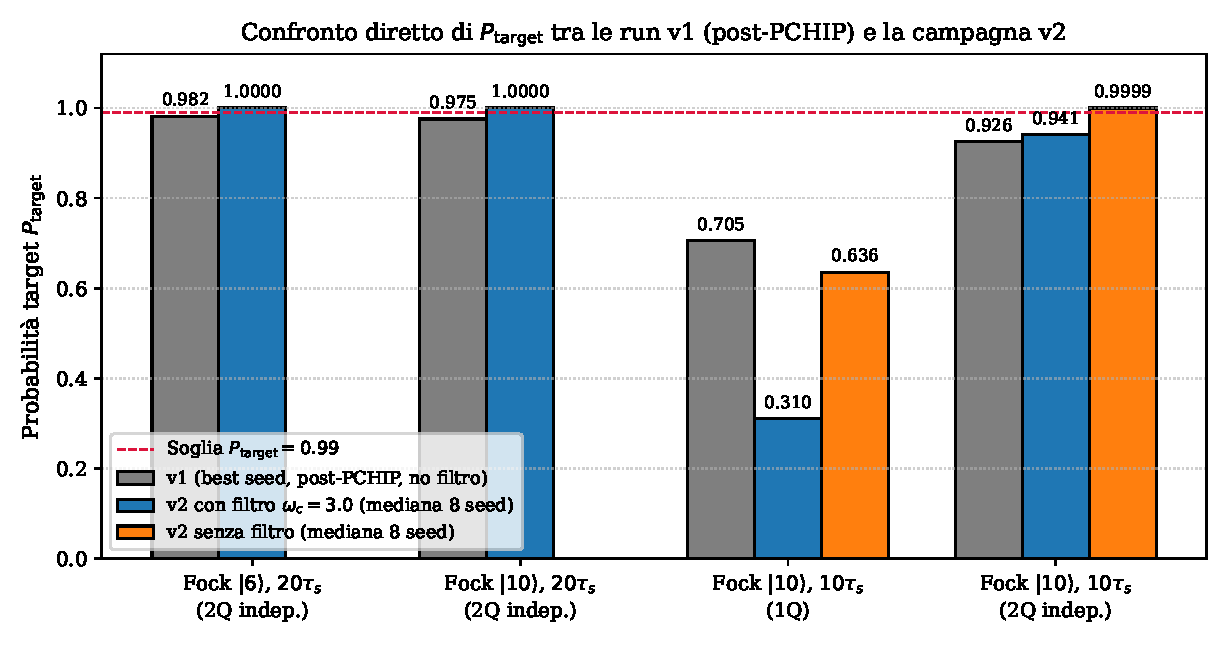
\includegraphics[width=0.76\textwidth]{figure/fig3_confronto_v1_v2.pdf}
    \caption{}
    \label{fig:confronto_v1_v2}
\end{figure}

\begin{table}[H]
\centering
\footnotesize
\setlength{\tabcolsep}{4pt}
\renewcommand{\arraystretch}{1.15}
\resizebox{\textwidth}{!}{%
\begin{tabular}{llccc}
\toprule
\textbf{Caso fisico} & \textbf{Metrica} & \textbf{v1 (1 seed, post-PCHIP)} & \textbf{v2 con filtro $3.0$ (8 seed)} & \textbf{v2 senza filtro (8 seed)} \\
\midrule
\multirow{2}{*}{\textbf{Fock $n=6$, $T=20\,\tau_s$ — 2Q ind.}}
 & $F_{\text{root}}$ (best / med.) & $0.990824$ (GRAPE $0.999967$) & $0.999999$ (med. $0.999998$) & — \\
 & $P_{\text{target}}$ (best / med.) & $\approx 0.9817$ & $0.999998$ (med. $0.999996$, \textbf{8/8}) & — \\
\midrule
\multirow{2}{*}{\textbf{Fock $n=10$, $T=20\,\tau_s$ — 2Q ind.}}
 & $F_{\text{root}}$ (best / med.) & $0.987673$ (GRAPE $0.999906$) & $0.999998$ (med. $0.999997$) & $0.999993$ (med. $0.999989$) \\
 & $P_{\text{target}}$ (best / med.) & $\approx 0.9755$ & $0.999995$ (med. $0.999994$, \textbf{8/8}) & $0.999987$ (med. $0.999979$, \textbf{8/8}) \\
\midrule
\multirow{2}{*}{\textbf{Fock $n=10$, $T=10\,\tau_s$ — 1Q}}
 & $F_{\text{root}}$ (best / med.) & $0.839708$ (GRAPE $0.872035$) & $0.593975$ (med. $0.5569$) & $0.838545$ (med. $0.7972$) \\
 & $P_{\text{target}}$ (best / med.) & $\approx 0.7051$ & $0.352806$ (med. $0.3102$, \textbf{0/8}) & $0.703158$ (med. $0.6355$, \textbf{0/8}) \\
\midrule
\multirow{2}{*}{\textbf{Fock $n=10$, $T=10\,\tau_s$ — 2Q ind.}}
 & $F_{\text{root}}$ (best / med.) & $0.962247$ (GRAPE $0.998764$) & $0.980704$ (med. $0.9700$) & $0.999985$ (med. $0.999968$) \\
 & $P_{\text{target}}$ (best / med.) & $\approx 0.9259$ & $0.961781$ (med. $0.9410$, \textbf{0/8}) & $0.999970$ (med. $0.999937$, \textbf{8/8}) \\
\bottomrule
\end{tabular}%
}
\caption{}
\label{tab:confronto_v1_v2}
\end{table}

\begin{itemize}
    \item \textbf{Eliminazione del crollo post-smoothing e coerenza fisica:} ottimizzando direttamente il comando continuo filtrato con gradiente esatto, in v2 sparisce la perdita del $2\%\text{--}7\%$ causata in v1 dallo smoothing PCHIP a posteriori. Sul caso 1Q a $10\,\tau_s$ senza filtro (\texttt{main\_010}), il miglior seed v2 riproduce lo stesso limite di v1 ($F_{\text{root}} = 0.8385$ vs $0.8397$).
    \item \textbf{Perché in v2 la fase CRAB si ferma a probabilità basse mentre in v1 arrivava a $F \approx 0.95\text{--}0.99$:}
    Nei report della v2 si nota che dopo il solo passo CRAB la probabilità target $P_{\text{CRAB}}$ è piccola (ad es.\ $\sim 10^{-4}\text{--}10^{-2}$ su $n=10$, per poi salire a $>0.99999$ in GRAPE), mentre in v1 CRAB arrivava a $F_{\text{root}} \approx 0.96\text{--}0.99$. Elenco di seguito le probabili cause:
    \begin{enumerate}
        \item In v1 la ricerca CRAB era completamente non vincolata e Nelder--Mead raggiungeva $F \approx 0.98$ solo spingendo i drive a escursioni non fisiche $\Omega_D/\omega_c \in [-2.8, +7.5]$ (incluse frequenze totali negative), che poi dovevano essere tagliate passandole a GRAPE in $[0.5, 3.0]$. In v2, invece, ogni tentativo CRAB viene riscalato globalmente da \texttt{feasible\_nodes} per restare sempre dentro i limiti fisici $\Omega_j(t) \in [0.5, 3.0]$ ($\delta_j \in [-1.5, +1.0]$): se la somma delle 20 armoniche presenta anche un solo picco sopra $+1.0$, l'intera forma d'onda viene contratta verso zero, limitando l'energia media.
        \item In v2 i coefficienti iniziali di Fourier sono estratti con deviazione standard piccola ($\sigma_0 = 0.1$, contro $[-0.5, 0.5]$ in v1) e Nelder--Mead ha un tetto fisso di $6000$ valutazioni (mentre in v1 \texttt{max\_iter=None} su 80 parametri arrivava a $16\,000$ valutazioni).
        \item In v1 CRAB riportava la radice $F_{\text{root}} = \sqrt{P}$, mentre le tabelle v2 riportano $P = F_{\text{root}}^2$.
    \end{enumerate}
\end{itemize}

\section{Ultime considerazioni, ottimizzazione dei tempi di calcolo e prossimi passi}

\subsection*{1. Questioni fisiche e numeriche emerse dalla campagna}
\begin{itemize}
    \item \textbf{Fallimento del check \texttt{time\_grid} nei tentativi che non raggiungono il target a $T=10\,\tau_s$:}
In tutti i casi a $T=10\,\tau_s$ dove l'ottimizzatore resta lontano da $P=0.99$ (\texttt{1q} e \texttt{2q\_normalized} in \texttt{main\_006}, \texttt{main\_008}, \texttt{main\_010}, e \texttt{2q} filtrati in \texttt{main\_008}), il controllo \texttt{time\_grid} fallisce perché la differenza di fedeltà tra il propagatore midpoint a $N=1000$ intervalli e l'evoluzione continua \texttt{sesolve} supera la soglia di $10^{-4}$. Probabilmente quando non riesce a salire di probabilità con una dinamica regolare, GRAPE spinge i nodi a variare rapidamente tra uno step e l'altro. Per quei casi comunque i numeri continui ($P_{\text{target}}$ da \texttt{sesolve}) indicano chiaramente che il target non viene raggiunto.
\item \textbf{Tenuta dello stato dopo $T$ (\texttt{hold\_time}):}
Nelle simulazioni v2 osservo il sistema per ulteriori $2\,\tau_s$ dopo $T$, con il comando in ingresso posto a zero (come mostrato nella parte destra della Figura~\ref{fig:dinamica_fock6_t10}). Tuttavia, in regime USC l'accoppiamento $g$ con i qubit resta attivo anche per $t>T$ e, con il filtro attivo, il comando effettivo presenta inoltre una coda esponenziale che si esaurisce durante l'hold. Di conseguenza, lo stato di Fock preparato a $t=T$ scambia rapidamente energia con i qubit e la probabilità $P_{\text{target}}$ può diminuire già durante l'hold, raggiungendo minimi compresi tra $\sim 0.02$ e $0.28$ per $n=6$ e $n=10$.
\end{itemize}

\subsection*{2. Possibili analisi sui dati già salvati}
Prima di avviare nuove campagne di simulazione possiamo usare i dati già salvati per simulare scenari più realistici:
\begin{enumerate}
    \item Applicare errori di offset statico, errori di guadagno e offset di fase sui due canali degli attuatori.
    \item Applicare a posteriori frequenze di taglio $\omega_{\text{cut}}$
    \item \text{Evoluzione dissipativa in sistema aperto}
\end{enumerate}

\subsection*{3. Considerazioni per ridurre i tempi di simulazioni per le run future}
\begin{enumerate}
    \item Taglio delle valutazioni CRAB da $6000$ a $1200\text{--}1500$: nella campagna la fase CRAB ha assorbito l'$83\%\text{--}92\%$ del tempo di calcolo (ad es.\ in \texttt{main\_009} su \texttt{2q\_independent}: $790\text{ min}$ per CRAB contro $146\text{ min}$ per GRAPE e $0.3\text{ min}$ per la validazione), perché ogni valutazione CRAB esegue $N=2000$ diagonalizzazioni midpoint. Il collaudo \texttt{pilot\_002} sullo stesso Fock $|10\rangle$ a $20\,\tau_s$ dimostra però che con sole $1200$ valutazioni CRAB e $80$ iterazioni GRAPE tutti i seed raggiungono già $P \ge 0.9990$ validato in $78\text{ min}$ invece di $898\text{ min}$ ($11.5\times$ più veloce).
    \item Riduzione delle iterazioni GRAPE da $600$ a $250\text{--}300$: analizzando il log dei risultati si osserva che in tutti i casi validati GRAPE supera la soglia $P \ge 0.99$ entro $10\text{--}70$ iterazioni, $P \ge 0.999$ entro $25\text{--}130$ iterazioni e $P \ge 0.9999$ entro $50\text{--}250$ iterazioni (a $300$ iterazioni la mediana è già $\ge 0.99996$). Le iterazioni $300\text{--}600$ servono solo a limare la quinta cifra decimale o, nei casi non validati a $10\,\tau_s$, ad accentuare le oscillazioni ad alta frequenza.
    \item Diminuire la dimensione dello spazio: per target con $\langle n\rangle \le 4$ (come Squeezed $3\text{ dB}$ e Cat $\alpha=2.0$), usare $\text{dim}=45\text{--}50$ (validato a $65\text{--}70$) invece di $60\to 80$.
\end{enumerate}

\subsection*{4. Cambiamenti al codice}
\begin{enumerate}
    \item Valutare CRAB su una griglia meno fine (es.\ $N_{\text{CRAB}} = 400\text{--}500$) passando alla griglia fine $N=2000$ solo in GRAPE.
    \item Fermare GRAPE quando $P_{\text{target}}$ supera una soglia di saturazione (es.\ $0.99995$) e introdurre un peso minimo $\texttt{slew\_weight} \sim 10^{-5}$ a $T=10\,\tau_s$.
    \item Includere direttamente $C_{2,\text{tot}}$ e $C_{2,\text{max ch}}$ nei JSON e nei CSV generati dalla pipeline.
\end{enumerate}

\noindent
Con queste modifiche, le future campagne di simulazione dovrebbero essere completate in $\sim 1/10$ del tempo della campagna v2 (tempo di simulazione di 11 giorni).\\

\noindent
Tutti i log e i dati ottenuti dalla simulazione sono salvati e disponibili per ulteriori analisi.

\newpage
\section{Campagna intermedia: ottimizzazioni di calcolo ed estensione a stati Cat e Squeezed}

Prima di passare all'introduzione del vincolo esplicito sullo slew rate, ho implementato nella pipeline \texttt{v2/qoc/} gli accorgimenti individuati alla fine della sezione precedente e ho eseguito una campagna intermedia completa (\texttt{campagna\_intermedia\_fock\_cat\_squeezed\_20261030T163304\_082788Z}, $17$ blocchi $\times 5$ sistemi $\times 8$ seed $= 680$ pipeline totali).

\subsection{Modifiche implementate e piano degli esperimenti}
\begin{enumerate}
    \item \textbf{Griglia temporale ridotta in CRAB (\texttt{crab\_intervals}) e budget \texttt{crab\_max\_eval = 1500}:} la fase esplorativa CRAB viene valutata su una griglia temporale ridotta di un fattore $4$ rispetto a GRAPE ($N_{\text{CRAB}} = N_{\text{GRAPE}}/4$, scalata automaticamente con la durata $T$: $250$, $375$ e $500$ intervalli midpoint per $T = 10, 15, 20\,\tau_s$), passando poi alla griglia fine ($1000$, $1500$, $2000$ intervalli) per il raffinamento locale con GRAPE.
    \item \textbf{Early stopping in GRAPE (\texttt{grape\_stop\_probability = 0.99995}):} il raffinamento con \texttt{L-BFGS-B} (tetto massimo ridotto da $600$ a $300$ iterazioni) si arresta automaticamente non appena la probabilità discreta supera $P_{\text{disc}} \ge 0.99995$, evitando iterazioni superflue in regime di saturazione.
    \item \textbf{Dimensione di Fock adattata per famiglia di stato e metriche $C_2$ native:} ho aggiunto il supporto per sovrascrivere \texttt{dimension} e \texttt{control} per singolo blocco della campagna, mantenendo $\text{dim}=60$ (validato a $\text{dim}=80$) per gli stati di Fock $|6\rangle$ e $|10\rangle$ e impostando $\text{dim}=48$ (validato a $\text{dim}=68$) per gli stati Cat ($\alpha=2.0$) e Squeezed ($3\,\text{dB}$ e $8\,\text{dB}$, con angolo $\theta = \pi/4$). I costi energetici del paper $C_{2,\text{tot}}$ e $C_{2,\text{max ch}}$ vengono ora salvati nativamente in tutti i file JSON e CSV.
\end{enumerate}

\noindent
La campagna intermedia esplora tre famiglie di stati non classici, affiancando alle simulazioni con filtro causale ($\omega_{\text{cut}} = 3.0\,\omega_c$, Tabella~\ref{tab:intermedia_filtrata}) un set sistematico di simulazioni di controllo senza filtro ($\omega_{\text{cut}} = \text{null}$, Tabella~\ref{tab:intermedia_nofiltro}):
\begin{itemize}
    \item \textbf{Stati di Fock ($\text{dim}=60 \to 80$):} verifica dei casi chiave della campagna precedente su $|n=6\rangle$ a $T=10\,\tau_s$ (con e senza filtro, \texttt{main\_000}--\texttt{main\_001}) e su $|n=10\rangle$ a $T=10, 20\,\tau_s$ (\texttt{main\_002}, \texttt{main\_004}, \texttt{main\_005}), più il nuovo punto intermedio a $T = 15\,\tau_s$ con filtro (\texttt{main\_003}).
    \item \textbf{Stati di Schrödinger Cat a 4 componenti ($\alpha = 2.0$, $\langle n \rangle = 4$, $\text{dim}=48 \to 68$):} scansione su tre durate $T = 10, 15, 20\,\tau_s$ con filtro (\texttt{main\_006}--\texttt{main\_008}) e controlli senza filtro a $T = 10, 15\,\tau_s$ (\texttt{main\_009}--\texttt{main\_010}).
    \item \textbf{Stati Squeezed Vacuum ($3\,\text{dB}$ e $8\,\text{dB}$, $\theta = \pi/4$, $\text{dim}=48 \to 68$):} confronto tra squeezing moderato ($3\,\text{dB}$, $r \approx 0.346$, $\langle n\rangle \approx 0.12$) e squeezing forte ($8\,\text{dB}$, $r \approx 0.921$, $\langle n\rangle \approx 1.11$) a $T = 10, 20\,\tau_s$ con filtro (\texttt{main\_011}--\texttt{main\_014}) e a $T = 10\,\tau_s$ senza filtro (\texttt{main\_015}--\texttt{main\_016}).
\end{itemize}

\begin{table}[H]
\centering
\scriptsize
\setlength{\tabcolsep}{3.2pt}
\renewcommand{\arraystretch}{1.08}
\resizebox{\textwidth}{!}{%
\begin{tabular}{llccccccc}
\toprule
\textbf{Esperimento} & \textbf{Sistema} & \textbf{Successi} & \textbf{$P_{\text{target}}$ med.} & \textbf{$P_{\text{target}}$ $[\min, \max]$} & \textbf{Fluenza $\mathcal{F}_{\text{mod}}$} & \textbf{Costo paper $C_2/\omega_c^2$} & \textbf{$\text{SR}_{\max}$ / $\omega_{99\%}$} & \textbf{Iter.\ GRAPE} \\
 & & \textbf{(valid.\ num.)} & \textbf{(continua)} & & \textbf{tot (max ch)} & \textbf{tot (max ch)} & \textbf{(mediana)} & \textbf{med.\ $[\min, \max]$} \\
\midrule
\multirow{5}{*}{\shortstack[l]{\textbf{Fock $|n=6\rangle$, $T=10\,\tau_s$}\\filtro $3.0$, $\text{dim}=60$ (\texttt{main\_000})}}
 & \texttt{1q} & 0/8 (0/8) & 0.717317 & $[0.617159, 0.748426]$ & $34.06$ ($34.06$) & $17.03$ ($17.03$) & $3.78$ / $4.74$ & $298$ $[206, 300]$ \\
 & \texttt{2q\_common} & 5/8 (7/8) & \textbf{0.993292} & $[0.973599, 0.999936]$ & $53.03$ ($26.51$) & $26.51$ ($13.26$) & $3.77$ / $5.46$ & $300$ $[300, 300]$ \\
 & \texttt{2q\_independent} & \textbf{8/8} (8/8) & \textbf{0.999942} & $[0.999874, 0.999948]$ & $48.16$ ($25.29$) & $24.08$ ($12.65$) & $3.73$ / $4.98$ & $300$ $[197, 300]$ \\
 & \texttt{2q\_norm\_common} & 0/8 (0/8) & 0.651781 & $[0.525758, 0.917784]$ & $79.07$ ($39.54$) & $39.54$ ($19.77$) & $3.78$ / $4.62$ & $300$ $[258, 300]$ \\
 & \texttt{2q\_norm\_independent} & 0/8 (0/8) & 0.738014 & $[0.384006, 0.768554]$ & $73.13$ ($37.44$) & $36.56$ ($18.72$) & $3.78$ / $4.74$ & $300$ $[300, 300]$ \\
\midrule
\multirow{5}{*}{\shortstack[l]{\textbf{Fock $|n=10\rangle$, $T=10\,\tau_s$}\\filtro $3.0$, $\text{dim}=60$ (\texttt{main\_002})}}
 & \texttt{1q} & 0/8 (0/8) & 0.302737 & $[0.158032, 0.400833]$ & $39.11$ ($39.11$) & $19.56$ ($19.56$) & $3.78$ / $4.74$ & $208$ $[151, 300]$ \\
 & \texttt{2q\_common} & 0/8 (0/8) & 0.882637 & $[0.763084, 0.947159]$ & $59.26$ ($29.63$) & $29.63$ ($14.81$) & $3.78$ / $5.04$ & $300$ $[167, 300]$ \\
 & \texttt{2q\_independent} & 0/8 (0/8) & 0.921985 & $[0.877577, 0.975032]$ & $65.43$ ($34.17$) & $32.72$ ($17.08$) & $3.78$ / $5.22$ & $300$ $[300, 300]$ \\
 & \texttt{2q\_norm\_common} & 0/8 (0/8) & 0.270133 & $[0.107894, 0.490162]$ & $75.16$ ($37.58$) & $37.58$ ($18.79$) & $3.78$ / $4.44$ & $256$ $[187, 300]$ \\
 & \texttt{2q\_norm\_independent} & 0/8 (0/8) & 0.354498 & $[0.233794, 0.466442]$ & $81.09$ ($43.26$) & $40.55$ ($21.63$) & $3.78$ / $4.68$ & $300$ $[300, 300]$ \\
\midrule
\multirow{5}{*}{\shortstack[l]{\textbf{Fock $|n=10\rangle$, $T=15\,\tau_s$}\\filtro $3.0$, $\text{dim}=60$ (\texttt{main\_003})}}
 & \texttt{1q} & 0/8 (0/8) & 0.937283 & $[0.872441, 0.973582]$ & $52.27$ ($52.27$) & $26.13$ ($26.13$) & $3.78$ / $4.84$ & $300$ $[219, 300]$ \\
 & \texttt{2q\_common} & \textbf{8/8} (8/8) & \textbf{0.999946} & $[0.999808, 0.999949]$ & $62.98$ ($31.49$) & $31.49$ ($15.75$) & $3.69$ / $5.04$ & $264$ $[196, 300]$ \\
 & \texttt{2q\_independent} & \textbf{8/8} (8/8) & \textbf{0.999945} & $[0.999943, 0.999946]$ & $65.08$ ($33.66$) & $32.54$ ($16.83$) & $3.68$ / $4.72$ & $204$ $[169, 300]$ \\
 & \texttt{2q\_norm\_common} & 0/8 (0/8) & 0.838046 & $[0.574137, 0.947635]$ & $95.02$ ($47.51$) & $47.51$ ($23.76$) & $3.78$ / $4.84$ & $300$ $[300, 300]$ \\
 & \texttt{2q\_norm\_independent} & 1/8 (1/8) & 0.979306 & $[0.810678, 0.992984]$ & $110.74$ ($56.80$) & $55.37$ ($28.40$) & $3.78$ / $4.80$ & $300$ $[300, 300]$ \\
\midrule
\multirow{5}{*}{\shortstack[l]{\textbf{Fock $|n=10\rangle$, $T=20\,\tau_s$}\\filtro $3.0$, $\text{dim}=60$ (\texttt{main\_004})}}
 & \texttt{1q} & \textbf{8/8} (8/8) & \textbf{0.999948} & $[0.999945, 0.999950]$ & $52.01$ ($52.01$) & $26.01$ ($26.01$) & $3.76$ / $4.68$ & $182$ $[152, 225]$ \\
 & \texttt{2q\_common} & \textbf{8/8} (8/8) & \textbf{0.999946} & $[0.999946, 0.999948]$ & $65.51$ ($32.75$) & $32.75$ ($16.38$) & $3.56$ / $4.32$ & $186$ $[127, 230]$ \\
 & \texttt{2q\_independent} & \textbf{8/8} (8/8) & \textbf{0.999946} & $[0.999944, 0.999948]$ & $54.25$ ($30.23$) & $27.13$ ($15.12$) & $3.61$ / $4.29$ & $176$ $[118, 218]$ \\
 & \texttt{2q\_norm\_common} & 6/8 (6/8) & \textbf{0.998454} & $[0.926864, 0.999860]$ & $117.09$ ($58.55$) & $58.55$ ($29.27$) & $3.78$ / $4.98$ & $300$ $[300, 300]$ \\
 & \texttt{2q\_norm\_independent} & \textbf{8/8} (8/8) & \textbf{0.999945} & $[0.999937, 0.999949]$ & $103.18$ ($54.42$) & $51.59$ ($27.21$) & $3.76$ / $4.77$ & $282$ $[198, 300]$ \\
\midrule
\multirow{5}{*}{\shortstack[l]{\textbf{Cat $\alpha=2.0$, $T=10\,\tau_s$}\\filtro $3.0$, $\text{dim}=48$ (\texttt{main\_006})}}
 & \texttt{1q} & 1/8 (6/8) & 0.977199 & $[0.951746, 0.992273]$ & $32.45$ ($32.45$) & $16.22$ ($16.22$) & $3.78$ / $4.80$ & $300$ $[300, 300]$ \\
 & \texttt{2q\_common} & \textbf{8/8} (8/8) & \textbf{0.999431} & $[0.997890, 0.999856]$ & $45.67$ ($22.84$) & $22.84$ ($11.42$) & $3.76$ / $5.28$ & $300$ $[300, 300]$ \\
 & \texttt{2q\_independent} & \textbf{8/8} (8/8) & \textbf{0.999838} & $[0.999489, 0.999906]$ & $47.28$ ($25.06$) & $23.64$ ($12.53$) & $3.77$ / $4.86$ & $300$ $[300, 300]$ \\
 & \texttt{2q\_norm\_common} & 0/8 (0/8) & 0.883836 & $[0.873494, 0.919944]$ & $64.95$ ($32.47$) & $32.47$ ($16.24$) & $3.78$ / $4.86$ & $300$ $[300, 300]$ \\
 & \texttt{2q\_norm\_independent} & 2/8 (3/8) & 0.979713 & $[0.956176, 0.998721]$ & $65.29$ ($33.94$) & $32.64$ ($16.97$) & $3.78$ / $5.04$ & $300$ $[300, 300]$ \\
\midrule
\multirow{5}{*}{\shortstack[l]{\textbf{Cat $\alpha=2.0$, $T=15\,\tau_s$}\\filtro $3.0$, $\text{dim}=48$ (\texttt{main\_007})}}
 & \texttt{1q} & \textbf{8/8} (8/8) & \textbf{0.999949} & $[0.999947, 0.999951]$ & $32.20$ ($32.20$) & $16.10$ ($16.10$) & $3.68$ / $4.68$ & $223$ $[127, 273]$ \\
 & \texttt{2q\_common} & \textbf{8/8} (8/8) & \textbf{0.999949} & $[0.999948, 0.999950]$ & $46.99$ ($23.50$) & $23.50$ ($11.75$) & $3.07$ / $4.08$ & $238$ $[187, 299]$ \\
 & \texttt{2q\_independent} & \textbf{8/8} (8/8) & \textbf{0.999949} & $[0.999862, 0.999950]$ & $38.61$ ($23.16$) & $19.30$ ($11.58$) & $3.20$ / $4.16$ & $294$ $[233, 300]$ \\
 & \texttt{2q\_norm\_common} & \textbf{8/8} (8/8) & \textbf{0.999399} & $[0.995952, 0.999910]$ & $83.96$ ($41.98$) & $41.98$ ($20.99$) & $3.74$ / $4.68$ & $300$ $[300, 300]$ \\
 & \texttt{2q\_norm\_independent} & \textbf{8/8} (8/8) & \textbf{0.999883} & $[0.999680, 0.999947]$ & $79.29$ ($42.38$) & $39.64$ ($21.19$) & $3.73$ / $4.84$ & $300$ $[300, 300]$ \\
\midrule
\multirow{5}{*}{\shortstack[l]{\textbf{Cat $\alpha=2.0$, $T=20\,\tau_s$}\\filtro $3.0$, $\text{dim}=48$ (\texttt{main\_008})}}
 & \texttt{1q} & \textbf{8/8} (8/8) & \textbf{0.999948} & $[0.999947, 0.999949]$ & $30.65$ ($30.65$) & $15.33$ ($15.33$) & $3.52$ / $4.14$ & $170$ $[122, 235]$ \\
 & \texttt{2q\_common} & \textbf{8/8} (8/8) & \textbf{0.999949} & $[0.999947, 0.999950]$ & $43.38$ ($21.69$) & $21.69$ ($10.84$) & $2.67$ / $3.75$ & $215$ $[185, 300]$ \\
 & \texttt{2q\_independent} & \textbf{8/8} (8/8) & \textbf{0.999949} & $[0.999948, 0.999950]$ & $35.31$ ($18.83$) & $17.66$ ($9.42$) & $2.65$ / $3.84$ & $241$ $[225, 290]$ \\
 & \texttt{2q\_norm\_common} & \textbf{8/8} (8/8) & \textbf{0.999947} & $[0.999920, 0.999949]$ & $72.35$ ($36.18$) & $36.18$ ($18.09$) & $3.65$ / $4.20$ & $278$ $[198, 300]$ \\
 & \texttt{2q\_norm\_independent} & \textbf{8/8} (8/8) & \textbf{0.999948} & $[0.999840, 0.999950]$ & $64.54$ ($35.00$) & $32.27$ ($17.50$) & $3.69$ / $4.02$ & $292$ $[174, 300]$ \\
\midrule
\multirow{5}{*}{\shortstack[l]{\textbf{Squeezed $3\,\text{dB}$, $T=10\,\tau_s$}\\filtro $3.0$, $\text{dim}=48$ (\texttt{main\_011})}}
 & \texttt{1q} & \textbf{8/8} (8/8) & \textbf{0.999953} & $[0.999950, 0.999964]$ & $5.54$ ($5.54$) & $2.77$ ($2.77$) & $1.67$ / $3.60$ & $34$ $[29, 39]$ \\
 & \texttt{2q\_common} & \textbf{8/8} (8/8) & \textbf{0.999951} & $[0.999950, 0.999953]$ & $13.36$ ($6.68$) & $6.68$ ($3.34$) & $1.45$ / $3.60$ & $35$ $[26, 39]$ \\
 & \texttt{2q\_independent} & \textbf{8/8} (8/8) & \textbf{0.999951} & $[0.999950, 0.999953]$ & $8.40$ ($4.74$) & $4.20$ ($2.37$) & $1.53$ / $3.54$ & $43$ $[39, 57]$ \\
 & \texttt{2q\_norm\_common} & \textbf{8/8} (8/8) & \textbf{0.999951} & $[0.999950, 0.999952]$ & $12.54$ ($6.27$) & $6.27$ ($3.14$) & $1.76$ / $3.60$ & $37$ $[31, 49]$ \\
 & \texttt{2q\_norm\_independent} & \textbf{8/8} (8/8) & \textbf{0.999953} & $[0.999950, 0.999955]$ & $9.39$ ($5.48$) & $4.70$ ($2.74$) & $1.40$ / $3.60$ & $46$ $[40, 52]$ \\
\midrule
\multirow{5}{*}{\shortstack[l]{\textbf{Squeezed $3\,\text{dB}$, $T=20\,\tau_s$}\\filtro $3.0$, $\text{dim}=48$ (\texttt{main\_012})}}
 & \texttt{1q} & \textbf{8/8} (8/8) & \textbf{0.999953} & $[0.999950, 0.999965]$ & $6.77$ ($6.77$) & $3.38$ ($3.38$) & $1.39$ / $3.66$ & $28$ $[23, 39]$ \\
 & \texttt{2q\_common} & \textbf{8/8} (8/8) & \textbf{0.999953} & $[0.999950, 0.999961]$ & $7.83$ ($3.91$) & $3.91$ ($1.96$) & $1.22$ / $3.09$ & $26$ $[15, 34]$ \\
 & \texttt{2q\_independent} & \textbf{8/8} (8/8) & \textbf{0.999952} & $[0.999950, 0.999955]$ & $10.23$ ($5.60$) & $5.12$ ($2.80$) & $1.39$ / $3.12$ & $33$ $[25, 39]$ \\
 & \texttt{2q\_norm\_common} & \textbf{8/8} (8/8) & \textbf{0.999951} & $[0.999950, 0.999952]$ & $12.88$ ($6.44$) & $6.44$ ($3.22$) & $1.28$ / $3.36$ & $42$ $[31, 56]$ \\
 & \texttt{2q\_norm\_independent} & \textbf{8/8} (8/8) & \textbf{0.999951} & $[0.999950, 0.999953]$ & $12.24$ ($6.41$) & $6.12$ ($3.20$) & $1.52$ / $3.24$ & $47$ $[45, 56]$ \\
\midrule
\multirow{5}{*}{\shortstack[l]{\textbf{Squeezed $8\,\text{dB}$, $T=10\,\tau_s$}\\filtro $3.0$, $\text{dim}=48$ (\texttt{main\_013})}}
 & \texttt{1q} & \textbf{8/8} (8/8) & \textbf{0.998505} & $[0.998025, 0.999255]$ & $27.64$ ($27.64$) & $13.82$ ($13.82$) & $3.75$ / $5.10$ & $300$ $[295, 300]$ \\
 & \texttt{2q\_common} & \textbf{8/8} (8/8) & \textbf{0.999404} & $[0.999055, 0.999621]$ & $36.25$ ($18.12$) & $18.12$ ($9.06$) & $3.71$ / $5.16$ & $300$ $[300, 300]$ \\
 & \texttt{2q\_independent} & \textbf{8/8} (8/8) & \textbf{0.999285} & $[0.998880, 0.999644]$ & $33.79$ ($17.98$) & $16.90$ ($8.99$) & $3.68$ / $5.28$ & $300$ $[300, 300]$ \\
 & \texttt{2q\_norm\_common} & \textbf{8/8} (8/8) & \textbf{0.998954} & $[0.998128, 0.999326]$ & $50.83$ ($25.42$) & $25.42$ ($12.71$) & $3.69$ / $4.92$ & $300$ $[300, 300]$ \\
 & \texttt{2q\_norm\_independent} & \textbf{8/8} (8/8) & \textbf{0.999400} & $[0.998095, 0.999610]$ & $50.82$ ($26.42$) & $25.41$ ($13.21$) & $3.70$ / $5.10$ & $300$ $[300, 300]$ \\
\midrule
\multirow{5}{*}{\shortstack[l]{\textbf{Squeezed $8\,\text{dB}$, $T=20\,\tau_s$}\\filtro $3.0$, $\text{dim}=48$ (\texttt{main\_014})}}
 & \texttt{1q} & \textbf{8/8} (8/8) & \textbf{0.999627} & $[0.999159, 0.999809]$ & $27.72$ ($27.72$) & $13.86$ ($13.86$) & $3.67$ / $4.68$ & $300$ $[300, 300]$ \\
 & \texttt{2q\_common} & \textbf{8/8} (8/8) & \textbf{0.999751} & $[0.999635, 0.999842]$ & $32.20$ ($16.10$) & $16.10$ ($8.05$) & $3.19$ / $4.92$ & $300$ $[300, 300]$ \\
 & \texttt{2q\_independent} & \textbf{8/8} (8/8) & \textbf{0.999607} & $[0.999461, 0.999771]$ & $30.22$ ($15.40$) & $15.11$ ($7.70$) & $3.41$ / $4.92$ & $300$ $[300, 300]$ \\
 & \texttt{2q\_norm\_common} & \textbf{8/8} (8/8) & \textbf{0.999647} & $[0.999511, 0.999841]$ & $55.25$ ($27.63$) & $27.63$ ($13.81$) & $3.55$ / $3.96$ & $300$ $[300, 300]$ \\
 & \texttt{2q\_norm\_independent} & \textbf{8/8} (8/8) & \textbf{0.999636} & $[0.999482, 0.999692]$ & $54.01$ ($30.02$) & $27.00$ ($15.01$) & $3.50$ / $4.02$ & $300$ $[300, 300]$ \\
\bottomrule
\end{tabular}%
}
\caption{Risultati della campagna intermedia per gli 11 blocchi con filtro passa-basso causale ($\omega_{\text{cut}} = 3.0\,\omega_c$).}
\label{tab:intermedia_filtrata}
\end{table}

\begin{table}[H]
\centering
\scriptsize
\setlength{\tabcolsep}{3.2pt}
\renewcommand{\arraystretch}{1.12}
\resizebox{\textwidth}{!}{%
\begin{tabular}{llccccccc}
\toprule
\textbf{Esperimento} & \textbf{Sistema} & \textbf{Successi} & \textbf{$P_{\text{target}}$ med.} & \textbf{$P_{\text{target}}$ $[\min, \max]$} & \textbf{Fluenza $\mathcal{F}_{\text{mod}}$} & \textbf{Costo paper $C_2/\omega_c^2$} & \textbf{$\text{SR}_{\max}$ / $\omega_{99\%}$} & \textbf{Iter.\ GRAPE} \\
 & & \textbf{(valid.\ num.)} & \textbf{(continua)} & & \textbf{tot (max ch)} & \textbf{tot (max ch)} & \textbf{(mediana)} & \textbf{med.\ $[\min, \max]$} \\
\midrule
\multirow{5}{*}{\shortstack[l]{\textbf{Fock $|n=6\rangle$, $T=10\,\tau_s$}\\senza filtro, $\text{dim}=60$ (\texttt{main\_001})}}
 & \texttt{1q} & 1/8 (1/8) & 0.981119 & $[0.956183, 0.999322]$ & $49.20$ ($49.20$) & $24.60$ ($24.60$) & $4.77$ / $8.16$ & $300$ $[235, 300]$ \\
 & \texttt{2q\_common} & \textbf{8/8} (8/8) & \textbf{0.999937} & $[0.999917, 0.999939]$ & $53.70$ ($26.85$) & $26.85$ ($13.42$) & $4.76$ / $7.80$ & $218$ $[179, 300]$ \\
 & \texttt{2q\_independent} & \textbf{8/8} (8/8) & \textbf{0.999938} & $[0.999929, 0.999941]$ & $54.19$ ($30.55$) & $27.09$ ($15.27$) & $4.76$ / $8.16$ & $176$ $[130, 214]$ \\
 & \texttt{2q\_norm\_common} & 0/8 (0/8) & 0.828066 & $[0.777615, 0.936965]$ & $97.49$ ($48.75$) & $48.75$ ($24.37$) & $4.77$ / $7.56$ & $300$ $[300, 300]$ \\
 & \texttt{2q\_norm\_independent} & 0/8 (0/8) & 0.976268 & $[0.887827, 0.995310]$ & $103.93$ ($54.05$) & $51.96$ ($27.03$) & $4.77$ / $7.44$ & $300$ $[300, 300]$ \\
\midrule
\multirow{5}{*}{\shortstack[l]{\textbf{Fock $|n=10\rangle$, $T=10\,\tau_s$}\\senza filtro, $\text{dim}=60$ (\texttt{main\_005})}}
 & \texttt{1q} & 0/8 (0/8) & 0.687505 & $[0.603246, 0.724137]$ & $52.88$ ($52.88$) & $26.44$ ($26.44$) & $4.77$ / $7.80$ & $190$ $[157, 300]$ \\
 & \texttt{2q\_common} & 3/8 (3/8) & \textbf{0.994516} & $[0.959896, 0.999734]$ & $79.74$ ($39.87$) & $39.87$ ($19.93$) & $4.77$ / $7.86$ & $300$ $[300, 300]$ \\
 & \texttt{2q\_independent} & \textbf{8/8} (8/8) & \textbf{0.999737} & $[0.998240, 0.999903]$ & $78.60$ ($40.65$) & $39.30$ ($20.33$) & $4.77$ / $8.04$ & $300$ $[300, 300]$ \\
 & \texttt{2q\_norm\_common} & 0/8 (0/8) & 0.502739 & $[0.383340, 0.638977]$ & $100.73$ ($50.37$) & $50.37$ ($25.18$) & $4.77$ / $7.68$ & $298$ $[240, 300]$ \\
 & \texttt{2q\_norm\_independent} & 0/8 (0/8) & 0.653033 & $[0.565350, 0.806457]$ & $104.43$ ($53.58$) & $52.21$ ($26.79$) & $4.77$ / $7.92$ & $300$ $[300, 300]$ \\
\midrule
\multirow{5}{*}{\shortstack[l]{\textbf{Cat $\alpha=2.0$, $T=10\,\tau_s$}\\senza filtro, $\text{dim}=48$ (\texttt{main\_009})}}
 & \texttt{1q} & \textbf{8/8} (8/8) & \textbf{0.999789} & $[0.997088, 0.999928]$ & $43.56$ ($43.56$) & $21.78$ ($21.78$) & $4.77$ / $7.74$ & $300$ $[300, 300]$ \\
 & \texttt{2q\_common} & 7/8 (7/8) & \textbf{0.999931} & $[0.999776, 0.999946]$ & $54.80$ ($27.40$) & $27.40$ ($13.70$) & $4.65$ / $7.14$ & $294$ $[209, 300]$ \\
 & \texttt{2q\_independent} & \textbf{8/8} (8/8) & \textbf{0.999941} & $[0.999934, 0.999944]$ & $45.76$ ($25.09$) & $22.88$ ($12.55$) & $4.70$ / $7.80$ & $285$ $[191, 300]$ \\
 & \texttt{2q\_norm\_common} & 3/8 (3/8) & 0.989409 & $[0.922015, 0.997865]$ & $89.97$ ($44.98$) & $44.98$ ($22.49$) & $4.77$ / $7.74$ & $300$ $[300, 300]$ \\
 & \texttt{2q\_norm\_independent} & \textbf{8/8} (8/8) & \textbf{0.999779} & $[0.999151, 0.999888]$ & $79.36$ ($41.00$) & $39.68$ ($20.50$) & $4.77$ / $7.98$ & $300$ $[300, 300]$ \\
\midrule
\multirow{5}{*}{\shortstack[l]{\textbf{Cat $\alpha=2.0$, $T=15\,\tau_s$}\\senza filtro, $\text{dim}=48$ (\texttt{main\_010})}}
 & \texttt{1q} & \textbf{8/8} (8/8) & \textbf{0.999942} & $[0.999941, 0.999943]$ & $32.73$ ($32.73$) & $16.37$ ($16.37$) & $4.56$ / $7.76$ & $130$ $[125, 175]$ \\
 & \texttt{2q\_common} & \textbf{8/8} (8/8) & \textbf{0.999944} & $[0.999940, 0.999945]$ & $42.10$ ($21.05$) & $21.05$ ($10.52$) & $3.55$ / $6.72$ & $189$ $[140, 253]$ \\
 & \texttt{2q\_independent} & \textbf{8/8} (8/8) & \textbf{0.999944} & $[0.999940, 0.999946]$ & $35.87$ ($19.65$) & $17.94$ ($9.83$) & $3.48$ / $6.60$ & $220$ $[131, 270]$ \\
 & \texttt{2q\_norm\_common} & 7/8 (7/8) & \textbf{0.999918} & $[0.999815, 0.999944]$ & $88.57$ ($44.28$) & $44.28$ ($22.14$) & $4.72$ / $7.52$ & $300$ $[201, 300]$ \\
 & \texttt{2q\_norm\_independent} & \textbf{8/8} (8/8) & \textbf{0.999942} & $[0.999888, 0.999944]$ & $73.66$ ($44.05$) & $36.83$ ($22.03$) & $4.63$ / $6.64$ & $250$ $[171, 300]$ \\
\midrule
\multirow{5}{*}{\shortstack[l]{\textbf{Squeezed $3\,\text{dB}$, $T=10\,\tau_s$}\\senza filtro, $\text{dim}=48$ (\texttt{main\_015})}}
 & \texttt{1q} & \textbf{8/8} (8/8) & \textbf{0.999954} & $[0.999950, 0.999959]$ & $5.84$ ($5.84$) & $2.92$ ($2.92$) & $1.72$ / $3.96$ & $31$ $[24, 34]$ \\
 & \texttt{2q\_common} & \textbf{8/8} (8/8) & \textbf{0.999951} & $[0.999950, 0.999959]$ & $12.78$ ($6.39$) & $6.39$ ($3.20$) & $1.76$ / $4.14$ & $35$ $[30, 44]$ \\
 & \texttt{2q\_independent} & \textbf{8/8} (8/8) & \textbf{0.999951} & $[0.999950, 0.999956]$ & $8.57$ ($4.87$) & $4.28$ ($2.44$) & $1.52$ / $3.96$ & $38$ $[30, 46]$ \\
 & \texttt{2q\_norm\_common} & \textbf{8/8} (8/8) & \textbf{0.999952} & $[0.999950, 0.999955]$ & $11.60$ ($5.80$) & $5.80$ ($2.90$) & $1.86$ / $3.78$ & $37$ $[32, 47]$ \\
 & \texttt{2q\_norm\_independent} & \textbf{8/8} (8/8) & \textbf{0.999950} & $[0.999950, 0.999955]$ & $9.98$ ($5.79$) & $4.99$ ($2.90$) & $1.72$ / $3.84$ & $40$ $[36, 48]$ \\
\midrule
\multirow{5}{*}{\shortstack[l]{\textbf{Squeezed $8\,\text{dB}$, $T=10\,\tau_s$}\\senza filtro, $\text{dim}=48$ (\texttt{main\_016})}}
 & \texttt{1q} & \textbf{8/8} (8/8) & \textbf{0.999550} & $[0.999173, 0.999677]$ & $33.96$ ($33.96$) & $16.98$ ($16.98$) & $4.77$ / $8.10$ & $300$ $[300, 300]$ \\
 & \texttt{2q\_common} & 6/8 (6/8) & \textbf{0.999720} & $[0.999618, 0.999906]$ & $40.60$ ($20.30$) & $20.30$ ($10.15$) & $4.72$ / $7.80$ & $300$ $[300, 300]$ \\
 & \texttt{2q\_independent} & \textbf{8/8} (8/8) & \textbf{0.999752} & $[0.999635, 0.999897]$ & $36.58$ ($20.85$) & $18.29$ ($10.42$) & $4.77$ / $8.10$ & $300$ $[300, 300]$ \\
 & \texttt{2q\_norm\_common} & \textbf{8/8} (8/8) & \textbf{0.999610} & $[0.999480, 0.999791]$ & $64.46$ ($32.23$) & $32.23$ ($16.11$) & $4.77$ / $7.68$ & $300$ $[300, 300]$ \\
 & \texttt{2q\_norm\_independent} & \textbf{8/8} (8/8) & \textbf{0.999727} & $[0.999616, 0.999795]$ & $60.13$ ($31.80$) & $30.07$ ($15.90$) & $4.77$ / $8.04$ & $300$ $[300, 300]$ \\
\bottomrule
\end{tabular}%
}
\caption{Risultati della campagna intermedia per i 6 blocchi diagnostici senza filtro ($\omega_{\text{cut}} = \text{null}$).}
\label{tab:intermedia_nofiltro}
\end{table}

\subsection{Considerazioni dettagliate sui risultati della campagna intermedia}

\begin{enumerate}
    \item \textbf{Verifica dello speed-up computazionale ($\sim 10\times$ per blocco rispetto alla campagna precedente):}
    L'intera campagna da $17$ esperimenti ($680$ pipeline) è terminata in $\sim 55{,}8$ ore di wall-clock ($\approx 2{,}3$ giorni, contro gli $11$ giorni richiesti dagli $8$ esperimenti della campagna precedente). L'uso di $N_{\text{CRAB}} = N_{\text{GRAPE}}/4$ e di $1500$ valutazioni ha abbattuto la quota del tempo CPU assorbita da CRAB dall'$85\%\text{--}92\%$ al $42{,}5\%$ ($191{,}2\,\text{h}$ CPU in CRAB contro $258{,}2\,\text{h}$ in GRAPE+validazione). Inoltre, l'early stopping a $P_{\text{disc}} \ge 0.99995$ si è attivato in $264$ pipeline su $680$, fermando GRAPE dopo sole $26\text{--}47$ iterazioni sugli stati Squeezed a $3\,\text{dB}$ e dopo $\sim 170\text{--}240$ iterazioni sui casi Fock $|10\rangle$ e Cat a $15\text{--}20\,\tau_s$, senza alcuna perdita di fedeltà né di tasso di successo rispetto alle run di riferimento.

    \item \textbf{Stati di Fock $|n=6\rangle$ e $|n=10\rangle$, e individuazione della soglia a $T = 15\,\tau_s$ (\texttt{main\_000}--\texttt{main\_005}):}
    \begin{itemize}
        \item I blocchi di verifica su Fock $|6\rangle$ a $T=10\,\tau_s$ (\texttt{main\_000} con filtro, \texttt{main\_001} senza filtro) e su Fock $|10\rangle$ a $T=10\,\tau_s$ e $20\,\tau_s$ (\texttt{main\_002}, \texttt{main\_004}, \texttt{main\_005}) riproducono esattamente il quadro fisico della prima campagna v2: a $T=10\,\tau_s$ su $|6\rangle$ con filtro, \texttt{2q\_independent} ottiene $8/8$ seed validati ($P_{\text{med}} = 0.999942$) mentre \texttt{1q} e i casi normalizzati restano a $0/8$ ($P_{\text{med}} \approx 0.65\text{--}0.74$). Anche senza filtro (\texttt{main\_001}), per $|6\rangle$ a $10\,\tau_s$ sia \texttt{2q\_common} sia \texttt{2q\_independent} raggiungono $8/8$ ($0.999938$), mentre \texttt{1q} valida solo $1/8$ seed ($P_{\text{med}} = 0.9811$) e i casi normalizzati restano a $0/8$.
        \item Il nuovo blocco intermedio su Fock $|10\rangle$ a $T = 15\,\tau_s$ con filtro $\omega_{\text{cut}} = 3.0\,\omega_c$ (\texttt{main\_003}) individua esattamente la finestra temporale in cui il vantaggio a 2 qubit su $10$ fotoni emerge \emph{anche in presenza del filtro passa-basso}: sia \texttt{2q\_common} sia \texttt{2q\_independent} centrano $8/8$ seed validati ($P_{\text{med}} = 0.999946$, fermandosi per early stopping a una mediana di $204$ iterazioni in \texttt{2q\_independent}), mentre il singolo qubit \texttt{1q} non supera mai la soglia ($0/8$, $P_{\text{med}} = 0.9373$, max $0.9736$) e i sistemi normalizzati si fermano a $0/8$ (\texttt{2q\_norm\_common}, $0.8380$) e $1/8$ (\texttt{2q\_norm\_independent}, $0.9793$). Questo conferma che l'aumento dell'accoppiamento collettivo $g_{\text{eff}} = \sqrt{2}g$ riduce di almeno il $25\%$ il tempo minimo necessario per preparare Fock $|10\rangle$ con controlli filtrati.
    \end{itemize}

    \item \textbf{Stati di Schrödinger Cat a 4 componenti ($\alpha = 2.0$, $\langle n \rangle = 4$, \texttt{main\_006}--\texttt{main\_010}):}
    \begin{itemize}
        \item \emph{Superamento definitivo del crollo post-PCHIP della v1:} nella v1 a $T = 15\,\tau_s$ la fedeltà sullo stato Cat crollava da $0.9995$ (GRAPE a gradini) a $\sim 0.895$ dopo lo smoothing PCHIP. Nella v2, ottimizzando direttamente il controllo continuo filtrato, a $T = 15\,\tau_s$ (\texttt{main\_007}) e a $T = 20\,\tau_s$ (\texttt{main\_008}) tutti e 5 i sistemi raggiungono $8/8$ seed validati con probabilità continue $P_{\text{target}} \approx 0.99995$ ($F_{\text{root}} \approx 0.99997$). Inoltre, \texttt{2q\_independent} riduce il costo massimo per singolo canale $C_{2,\text{max ch}}$ del $28\%\text{--}39\%$ rispetto a \texttt{1q} ($11.58$ contro $16.10$ a $15\,\tau_s$; $9.42$ contro $15.33$ a $20\,\tau_s$) e abbassa lo slew rate mediano da $3.52\text{--}3.68$ a $2.65\text{--}3.20$.
        \item \emph{Natura del vantaggio a 2 qubit a $T = 10\,\tau_s$ (filtro vs limite di velocità quantistica):} a durata breve $T = 10\,\tau_s$ con filtro (\texttt{main\_006}), \texttt{2q\_common} e \texttt{2q\_independent} centrano $8/8$ seed ($P_{\text{med}} = 0.999431$ e $0.999838$, con costo per canale dimezzato a $11.4\text{--}12.5$), mentre \texttt{1q} si ferma a $1/8$ ($P_{\text{med}} = 0.9772$), \texttt{2q\_norm\_common} a $0/8$ ($0.8838$) e \texttt{2q\_norm\_independent} a $2/8$ ($0.9797$). Tuttavia, confrontando con il controllo senza filtro a $T = 10\,\tau_s$ (\texttt{main\_009}), si osserva che rimuovendo il filtro sia \texttt{1q} sia \texttt{2q\_norm\_independent} salgono a $8/8$ seed validati ($P_{\text{med}} = 0.999789$ e $0.999779$), ma per farlo devono sfruttare componenti ad alta frequenza ($\omega_{99\%} \approx 7.74\text{--}7.98\,\omega_c$, slew rate $4.77$). Ciò dimostra una differenza fisica importante rispetto a Fock $|6\rangle$ e $|10\rangle$: per lo stato Cat ($\langle n \rangle = 4$), a $T = 10\,\tau_s$ un accoppiamento efficace $g_{\text{eff}} = 0.3$ non è intrinsecamente troppo lento, ma richiede una modulazione rapida che viene tagliata dal filtro passa-basso a $3\,\omega_c$; l'accoppiamento collettivo $\sqrt{2}g$ dei due qubit permette invece di completare la sintesi dello stato Cat in $10\,\tau_s$ restando interamente dentro la banda del filtro ($\omega_{99\%} = 4.86\,\omega_c$).
    \end{itemize}

    \item \textbf{Stati Squeezed Vacuum a $3\,\text{dB}$ e $8\,\text{dB}$ (\texttt{main\_011}--\texttt{main\_016}) e diagnostica sul troncamento della coda fotonica:}
    \begin{itemize}
        \item \emph{Squeezed $3\,\text{dB}$ ($r \approx 0.346$, $\langle n \rangle \approx 0.12$, \texttt{main\_011}, \texttt{main\_012}, \texttt{main\_015}):} essendo molto vicino al vuoto, viene preparato da tutti i 5 sistemi con $8/8$ successi già a $T = 10\,\tau_s$ con filtro, attivando l'early stopping ($P \ge 0.99995$) in sole $26\text{--}47$ iterazioni GRAPE, con costi energetici minimi ($C_2 \approx 2.8\text{--}6.7$) e spettri naturalmente contenuti sotto la frequenza di taglio ($\omega_{99\%} \approx 3.1\text{--}3.7\,\omega_c$, slew rate $1.2\text{--}1.8$).
        \item \emph{Squeezed $8\,\text{dB}$ ($r \approx 0.921$, $\langle n \rangle \approx 1.11$, \texttt{main\_013}, \texttt{main\_014}, \texttt{main\_016}):} con filtro attivo tutti i sistemi raggiungono $8/8$ seed validati sia a $10\,\tau_s$ sia a $20\,\tau_s$; a $T = 10\,\tau_s$ (\texttt{main\_013}) i sistemi a 2 qubit raggiungono mediane più elevate rispetto a \texttt{1q} ($0.9993\text{--}0.9994$ contro $0.9985$) e riducono il carico energetico per canale del $35\%\text{--}44\%$ ($C_{2,\text{max ch}} \approx 9.0$ a $10\,\tau_s$ e $7.7\text{--}8.1$ a $20\,\tau_s$, contro $13.8\text{--}13.9$ di \texttt{1q}).
        \item \emph{Nota tecnica per il futuro sul troncamento di Fock per Squeezed $\ge 8\,\text{dB}$:} a differenza del caso a $3\,\text{dB}$, su $8\,\text{dB}$ tutte le pipeline arrivano al limite di $300$ iterazioni senza toccare la soglia di early stopping $0.99995$ (saturando a $P \approx 0.9993\text{--}0.9998$). Sebbene il numero medio di fotoni sia basso ($\langle n \rangle \approx 1.11$), la distribuzione sui livelli pari di uno stato Squeezed decade lentamente ($\propto \tanh^{2m} r$) e a $8\,\text{dB}$ presenta una coda non trascurabile fino a $n \approx 36\text{--}44$: a $\text{dim}=48$ la popolazione residua sui livelli di bordo è $\sim 3\times 10^{-5}$ e la distanza in traccia rispetto alla validazione a $\text{dim}=68$ è $\sim 2.4\times 10^{-4}$ (sotto la soglia di tolleranza $10^{-3}$, ma sufficiente a limitare la quarta cifra decimale di $P_{\text{target}}$). In particolare, nel controllo senza filtro a $T = 10\,\tau_s$ (\texttt{main\_016}), $2$ seed su $8$ di \texttt{2q\_common} raggiungono $P > 0.9997$ ma non superano il test \texttt{dimension\_convergence} ($1.04\times 10^{-3}$ e $1.23\times 10^{-3} > 10^{-3}$) perché i picchi ad alta frequenza non filtrati popolano transitoriamente la coda oltre $n=48$. Per future simulazioni su stati Squeezed a $8\,\text{dB}$ (o superiori) sarà quindi opportuno adottare $\text{dim}=60\text{--}64$ (validato a $\text{dim}=80\text{--}84$).
    \end{itemize}

    \item \textbf{Indicazioni per il prossimo passo (introduzione del vincolo sullo slew rate):}
    Dai dati raccolti finora emerge che il filtro causale a $\omega_{\text{cut}} = 3.0\,\omega_c$ contiene già la banda a $\omega_{99\%} \approx 3.1\text{--}5.3\,\omega_c$, ma nei regimi rapidi ($T = 10\text{--}15\,\tau_s$) l'ottimizzatore spinge comunque la pendenza istantanea del comando al massimo consentito dalla risposta esponenziale del filtro ($\text{SR}_{\max} \approx 3.68\text{--}3.78\,\omega_c^2$, contro $\approx 4.77\,\omega_c^2$ senza filtro). Nella prossima fase potremo quindi attivare la penalità esplicita sullo slew rate (\texttt{slew\_weight}) sui casi più significativi (Fock $|6\rangle$ a $10\,\tau_s$, Fock $|10\rangle$ a $15\text{--}20\,\tau_s$, Cat $\alpha=2.0$ a $10\text{--}15\,\tau_s$ e Squeezed $8\,\text{dB}$ con $\text{dim}=60$), verificando se la ripartizione del drive sui due canali di \texttt{2q\_independent} consenta di mantenere $P_{\text{target}} \ge 0.99$ anche imponendo rampe di frequenza significativamente più dolci rispetto al singolo qubit.
\end{enumerate}

\end{document}
